%% ****** Start of file aiptemplate.tex ****** %
%%
%%   This file is part of the files in the distribution of AIP substyles for REVTeX4.
%%   Version 4.1 of 9 October 2009.
%%
%
% This is a template for producing documents for use with 
% the REVTEX 4.1 document class and the AIP substyles.
% 
% Copy this file to another name and then work on that file.
% That way, you always have this original template file to use.

%\documentclass[aip,graphicx]{revtex4-1}
%\documentclass[aip,reprint]{revtex4-1}

%\usepackage{graphicx}

%\draft % marks overfull lines with a black rule on the right
%\documentclass[pre,aps,floatfix,authordate1-4,twocolumn]{revtex4-1}
%\documentclass[pre,aps,floatfix,authordate1-4]{revtex4-1}

\documentclass[aps,prl,superscriptaddress,twocolumn]{revtex4}



%\documentclass[aps,prl,preprint,groupedaddress]{revtex4}

\usepackage{rotating} 
\usepackage{times}
\usepackage{graphicx}
\usepackage{setspace}
\usepackage{amsmath}
\usepackage{epstopdf}
\usepackage[obeyFinal]{easy-todo}
\usepackage{csquotes}
\usepackage{xr}
\externaldocument{manuscriptPGPEsuppl}


\begin{document}

% Use the \preprint command to place your local institutional report number 
% on the title page in preprint mode.
% Multiple \preprint commands are allowed.
%\preprint{}

\title{NMRlipids IV: Headgroup \& glycerol backbone structures, and cation binding in bilayers with PE and PG lipids} %Title of paper

% repeat the \author .. \affiliation  etc. as needed
% \email, \thanks, \homepage, \altaffiliation all apply to the current author.
% Explanatory text should go in the []'s, 
% actual e-mail address or url should go in the {}'s for \email and \homepage.
% Please use the appropriate macro for the type of information

% \affiliation command applies to all authors since the last \affiliation command. 
% The \affiliation command should follow the other information.

\author{Pavel Buslaev}
\affiliation{University of Jyv{\"a}skyl{\"a}}

\author{Fernando Favela-Rosales}
\affiliation{Departamento de Investigaci\'{o}n, Tecnol\'{o}gico Nacional de M\'{e}xico, Campus Zacatecas Occidente, M\'{e}xico}

\author{Patrick Fuchs}
\affiliation{Paris, France}

\author{Matti Javanainen}
\affiliation{Institute of Organic Chemistry and Biochemistry of the 
Czech Academy of Sciences, Flemingovo n\'{a}m. 542/2, CZ-16610 Prague 6, Czech Republic}

\author{Jesper J. Madsen}
\affiliation{Department of Chemistry, The University of Chicago, Chicago, Illinois, United States of America}
\affiliation{Department of Global Health, College of Public Health, University of South Florida, Tampa, Florida, United States of America}

\author{Josef Melcr}
\affiliation{Institute of Organic Chemistry and Biochemistry of the 
Czech Academy of Sciences, Flemingovo n\'{a}m. 542/2, CZ-16610 Prague 6, Czech Republic}
\affiliation{Groningen Biomolecular Sciences and Biotechnology Institute 
and The Zernike Institute for Advanced Materials, 
University of Groningen, 9747 AG Groningen, The Netherlands}


\author{Markus S. Miettinen}
% \affiliation[Max Planck Institute of Colloids and Interfaces]{Department of Theory and Bio-Systems, Max Planck Institute of Colloids and Interfaces, 14424 Potsdam, Germany}
\affiliation{Department of Theory and Bio-Systems, Max Planck Institute of Colloids and Interfaces, 14424 Potsdam, Germany}

\author{O. H. Samuli Ollila}
\email[]{samuli.ollila@helsinki.fi}
\affiliation{Institute of Biotechnology, University of Helsinki}

\author{Chris G. Papadopoulos}
\affiliation{I2BC - University Paris Sud}


\author{Antonio Pe{\'o}n}
\affiliation{Spain}

\author{Thomas J. Piggot}
\affiliation{Chemistry, University of Southampton, Highfield, Southampton SO17 1BJ, United Kingdom}

\author{Pierre Poulain}
\affiliation{Paris, France}

% Collaboration name, if desired (requires use of superscriptaddress option in \documentclass). 
% \noaffiliation is required (may also be used with the \author command).
%\collaboration{}
%\noaffiliation

\date{\today}

\begin{abstract}
% insert abstract here
Abstract
\end{abstract}

%\pacs{}% insert suggested PACS numbers in braces on next line

\maketitle %\maketitle must follow title, authors, abstract and \pacs

% Body of paper goes here. Use proper sectioning commands. 
% References should be done using the \cite, \ref, and \label commands


%\label{}
\section{Introduction}

PE and PG lipids are most common lipids in bacteria \cite{sohlenkamp16}.
Zwitterionic PE is the second most abundant glycerophospholipid in eukaryotic cells
and has been related to the diseases \cite{vance15,calzada16,patel17}.
Anionic PG lipids are less abundant, but is also proposed to be fundamental for terrestrial life \cite{furse17}.
PE and PG affect membrane protein functionality \cite{hariharan18} and bind to various proteins \cite{yeagle14}.
PE headgroup is also prone for negative membrane curvature and causes membrane fusion \cite{Chernomordik08,calzada16}.
Therefore, the PE and PG headgroup structures play probably essential roles in 
many biological processes.

Structural details of lipid headgroups are mainly studied using NMR experiments, which
suggest that the glycerol backbone structures are largely similar irrespectively of the headroup \cite{gally81}, 
glycerol backbone and headgroup structure and behaviour are similar in model membranes and in bacteria \cite{gally81,scherer87,seelig90},
and the headgroup structures are similar in PC, PE and PG lipids, while headgroup is more rigid in PS lipids \cite{wohlgemuth80,buldt81}. 
%Extensive discussion about structural details of PE, PG or PS headgroups do not exists (as far as I know), 
%In contrast to PC lipids (see \cite{botan15} and references therein).
Some attempts to resolve conformational ensembles from NMR for PC and PE lipids have been made,
but lesser extend for PG or PS lipids \cite{seelig77c,davis83,Semchyschyn04}.
Classical molecular dynamics simulations could potentially give such ensembles and therefore enable
the detailed studies of lipid headgroup behaviour in complex biomolecular systems, but current
force fields are not accurate enough to reproduce the correct conformational ensembles for PC and PS headgroups \cite{botan15,antila19}.
Several MD simulations of PE and PG lipids have been published especially in the context of modeling
inner membrane of Gram-negative
bacteria \cite{devries04,murzyn05,pedersen06,zhao07,gurtovenko08,zhao08,henin09,kukol09,tsai12,dickson12,venable13,dickson14,berglund15}
\todo{There may be some relevant publication missing from here},
but evaluation of glycerol backbone and headgroup structures against experiments is rare \cite{henin09}.

Derivation of different lipid headgroup conformational ensembles in liquid state has been
inconclusive due to lack of suitable experimental data and tools to interpret the conformational ensembles.


Besides the structure, also ion binding may regulate biophysical activity of especially negatively
charged lipid headgroups \cite{seelig90}. Monovalent cation (except Lithium) binding to zwitterionic PC and anionic PS headgroups is
very weak, while multivalent ion binding is stronger but still weak \cite{cevc90,tocanne90,roux90,catte16,antila19}. The ion binding affinity
data for PE is more scarce \cite{marra85}, but large differences to PC would be surprising.
Negatively charged lipids are suggested to bear same cation binding constants than zwitterionic lipids, but
the amount of bound ions to negatively charged membranes would still be larger because
the concentration of cations in the vicinity of membranes would be higher  \cite{seelig90}.
%is stronger
%Based on the electrometer concept and other data is has been suggested that \cite{seelig90}
%\begin{displayquote}
%  {\it ''(i) Ca$^{2+}$ binds to neutral lipids (phosphatidylcholine, phosphatidylethanolamine) and negatively charged lipids
%    (phosphatidylglycerol) with approximately the same binding constant of K = 10-20 M$^{-1}$; \\
%    (ii) the free Ca$^{2+}$
%    concentration at the membrane interface is distinctly enhanced if the membrane carries a negative surface
%    charge, either due to protein or to lipid; \\
%    (iii) increased inter-facial Ca$^{2+}$ also means increased amounts
%    of bound Ca$^{2+}$ at neutral and charged lipids; \\
%    (iv) the actual binding step can be described by a Langmuir
%    adsorption isotherm with a 1 lipid:1 Ca$^{2+}$ stoichiometry, provided the interfacial concentration C$_M$, is
%    used to describe the chemical binding equilibrium.''}
%\end{displayquote}
On the other hand, anionic PS lipids are proposed chelate with calcium ions \cite{hauser85,feigenson86,roux91}.
In simulations, the cation binding affinity to PC and PS membranes is typically overestimated \cite{catte16,antila19},
which can be improved by applying the ECC to the partial charges of the force fields \cite{melcr18,melcr19}.

Here, we use open collaboration and order parameters of glycerol backbone and headgroup
to evaluate the accuracy of PE and PG heagroup structures, and the cation binding affinity

to anionic membranes containing PG lipids in the current MD simulation force fields.
The force field giving the best description for glycerol backbone and headgroup structures
of PC, PS, PG and PE headgroups (CHARMM36) reproduces the essential differences in order parameters
between these headgroups, and therefore enables the analysis of structural differences between the
headgroups.

%\begin{figure}[]
%  \centering
%  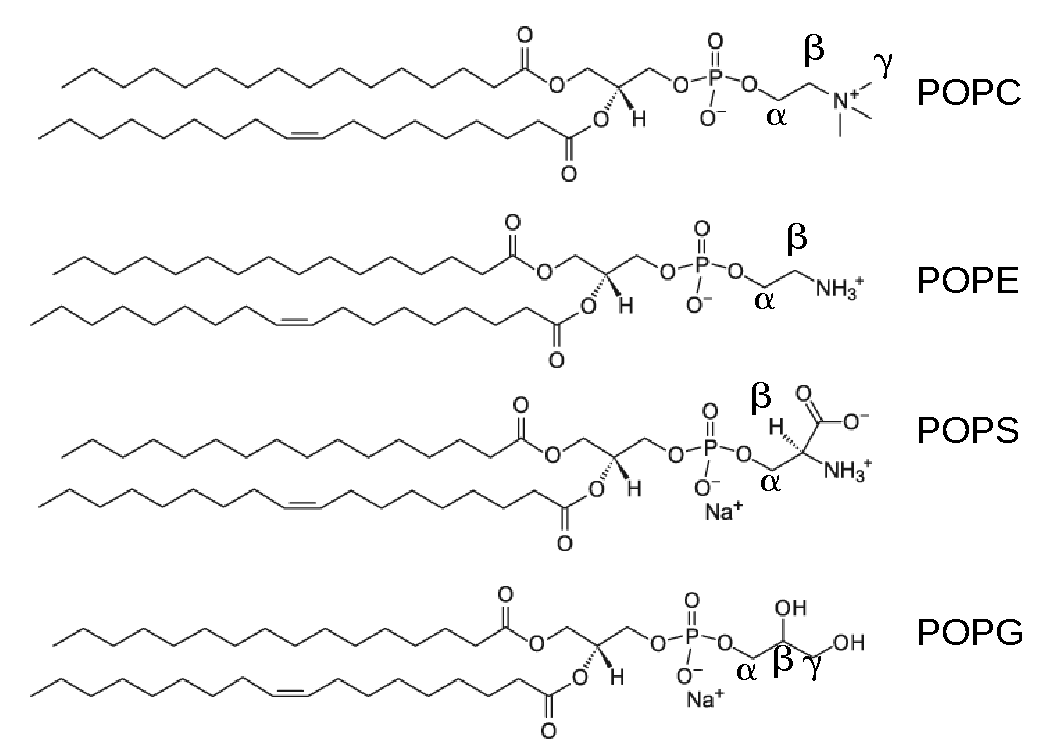
\includegraphics[width=9.0cm]{../Figs/lipids.pdf}
%  \caption{\label{lipids}
%    Chemical structures and labels for the headgroup carbons.
%  }
%\end{figure}



\section{Methods}
\subsection{Experimental C--H bond order parameters}
The headgroup and glycerol backbone C--H bond order parameter magnitudes and signs of POPE and POPG
were determined by measuring the chemical-shift resolved dipolar splittings
with a R-type Proton Detected Local Field (R-PDLF) experiment~\cite{dvinskikh04} and
%The corresponding order parameter signs were measured with a
S-DROSS experiments~\cite{gross97} using natural abundance $^{13}$C solid state NMR spectroscopy
as described previously \cite{ferreira13,ferreira16}.
%The experiments were done in a Bruker Avance III 400 spectrometer operating at a $^1$H Larmor frequency of 400.03 MHz.
%Magic angle spinning (MAS) of the sample was used at a frequency of 5.15 kHz (R-PDLF experiment) and 5 kHz (S-DROSS experiment).
%The following experimental setups were used.
POPE and POPG powder were purchased from Avanti polar lipids.
The NMR experiments were identical to our previous work~\cite{antila19}.
\todo{Is this enough and correct, or should we repeat some methods from the NMRlipidsIVps paper?}
The POPE experiments were recorded at 310~K and POPG experiments at 298~K, where the bilayers are in the liquid disordered phase \cite{marsh13}.

Absolute values of the headgroup and glycerol backbone order parameters from PE and PG lipids are measured
previously using $^2$H NMR~\cite{seelig76,gally81,wohlgemuth80,borle85}. Because also the order parameter
signs bear essential information about the lipid structures \cite{botan15,ollila16}, we measured the
magnitudes and signs of POPE and POPG C--H bond headgroup and glycerol backbone order parameter in liquid phase
using the 2D-RPDLF and S-DROSS experiments, as described previously \cite{ferreira13,ferreira16,antila19}.
For POPE, the glycerol backbone and $\alpha$-carbon peaks in INEPT spectra were assigned based on
previously measured POPC spectra~\cite{ferreira13} and
the $\beta$-carbon peak was assigned based on $^{13}$C chemical shift table for amines available
at \url{https://www.chem.wisc.edu/areas/reich/nmr/c13-data/cdata.htm} (Fig. \ref{POPEspectra}).
For POPG, the glycerol backbone peaks in INEPT spectra were assigned based on
previously measured POPC spectra~\cite{ferreira13}, while $\alpha$ and  $\gamma$-carbon peaks
\todo{How were these assigned?} (Fig. \ref{POPGspectra}). The numerical value of the $\beta$-carbon
order parameter could not be determined, because its peak overlapped with the g$_2$ peak from glycerol backbone in POPG.
However, the order parameter of $\beta$-carbon is expected to be clearly smaller than for g$_2$
based on previous $^2$H NMR measurements \cite{wohlgemuth80,gally81,borle85}.
Therefore, the beginning of the S-DROSS curve gives the sign for g$_2$ order parameter and end for $\beta$ (Fig. \ref{POPGspectra} (E)).
This is confirmed with SIMPSON calculations using negative value for g$_2$ and positive value for $\beta$ order parameter (Fig. \ref{POPGsimpson}).
\todo{Details to be checked by Tiago}.

\subsection{Molecular dynamics simulations}

Molecular dynamics simulation data were collected using
the Open Collaboration method \cite{botan15}, with
the NMR\-lipids Project blog (\url{nmrlipids.blogspot.fi}) and
GitHub repository (\url{github.com/NMRlipids/NMRlipidsIVotherHGs})
as the communication platforms.
The simulated systems of pure PE and PG bilayers without additional ions
are listed in Tables \ref{systemsPE} and \ref{systemsPG},
and lipid mixtures with additional ions in Table~\ref{systemsMIX}.
Further simulation details are given in the SI, and
the simulation data are indexed in a
searchable database available at \url{www.nmrlipids.fi},
and in the NMRlipids/MATCH repository (\url{github.com/NMRlipids/MATCH}).

The C--H bond order parameters were calculated directly
from the carbon and hydrogen positions using the definition
\begin{equation}
S_{\rm CH}=\frac{1}{2}\langle 3\cos^2\theta -1 \rangle,
\end{equation}
where $\theta$ is the angle between the C--H bond and the membrane normal
(taken to align with $z$, with bilayer periodicity in the $xy$-plane).
Angular brackets denote average over all sampled configurations.
The order parameters were first calculated averaging over time separately
for each lipid in the system. The average and
the standard error of the mean were then calculated over different lipids.
Python programs that use the MDAnalysis library \cite{agrawal11,gowers16}
used for all atom simulations is available in Ref. \citenum{MATCHgit}
({\tt scripts/calcOrderParameters.py}). For united atom simulations, the trajectories
with hydrogens having ideal geometry were constructed first using either buildH program~\cite{buildH}
or ({\tt scratch/opAAUA\_prod.py}) in  Ref. \citenum{MATCHgit}, and the order parameters were
then calculated from these trajectories. This approach has been tested against trajectories
with explicit hydrogens and the deviations in order parameters are small \cite{buildH,piggot17}.\\
\todo{BuildH program is now cited with a direct link to the GitHub repo. I think that a release to Zenodo would be nice in the final publication.}\\
\todo{Maybe we should also shortly discuss here about the reasons for slight dependence of order parameter values on the method used to reconstruct hydrogens?}\\
The ion number density profiles were calculated using the {\tt gmx density} tool
of the Gromacs sofware package \cite{gromacsMANUAL}.

\subsection{Analysis of molecular dynamics simulation data}
The big data set of MD simulations was analysed in the NMRlipids databank manner.
Unique naming convention for lipid atoms in each force field was defined using the mapping files
and analysis for all simulations indexed in NMRlipids databank manner were performed
using python codes.

\subsection{Analysis of lipid conformations bound to proteins}
Dihedral angles of all available conformations in the PDB databank were calculated using the
API access to the databank.

%\clearpage
\begin{figure*}[]
  \centering
%  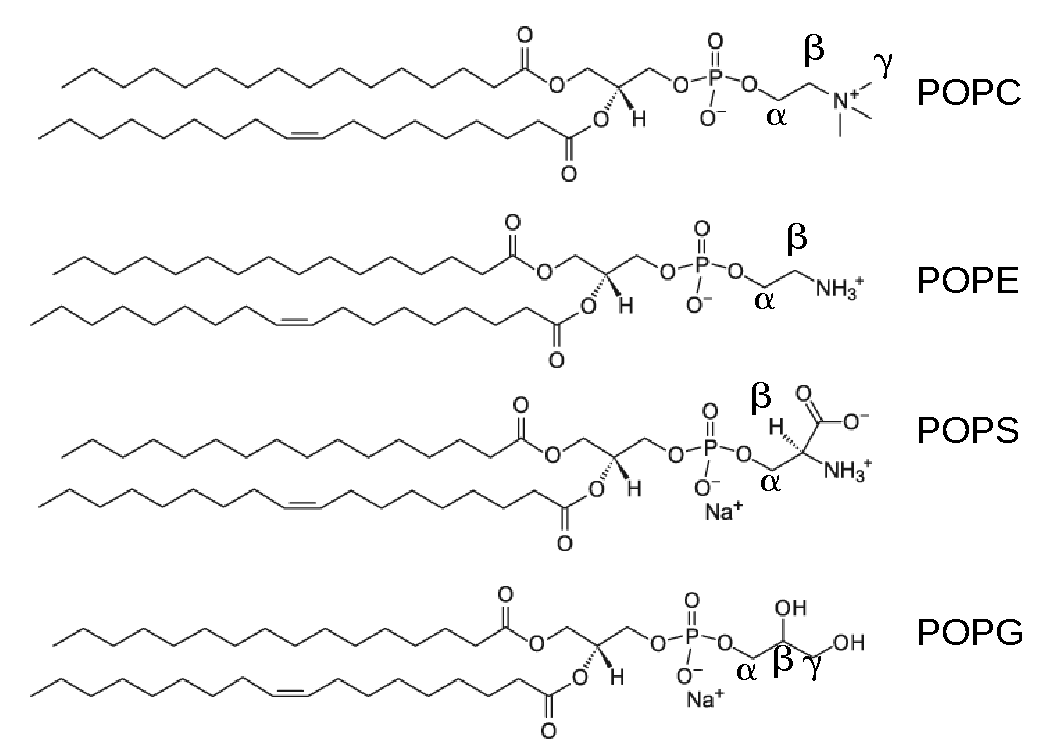
\includegraphics[width=9.0cm]{../Figs/lipids.pdf}
  %  \includegraphics[width=9.0cm]{../Figs/HGorderparametersPCPSPEPG.eps}
   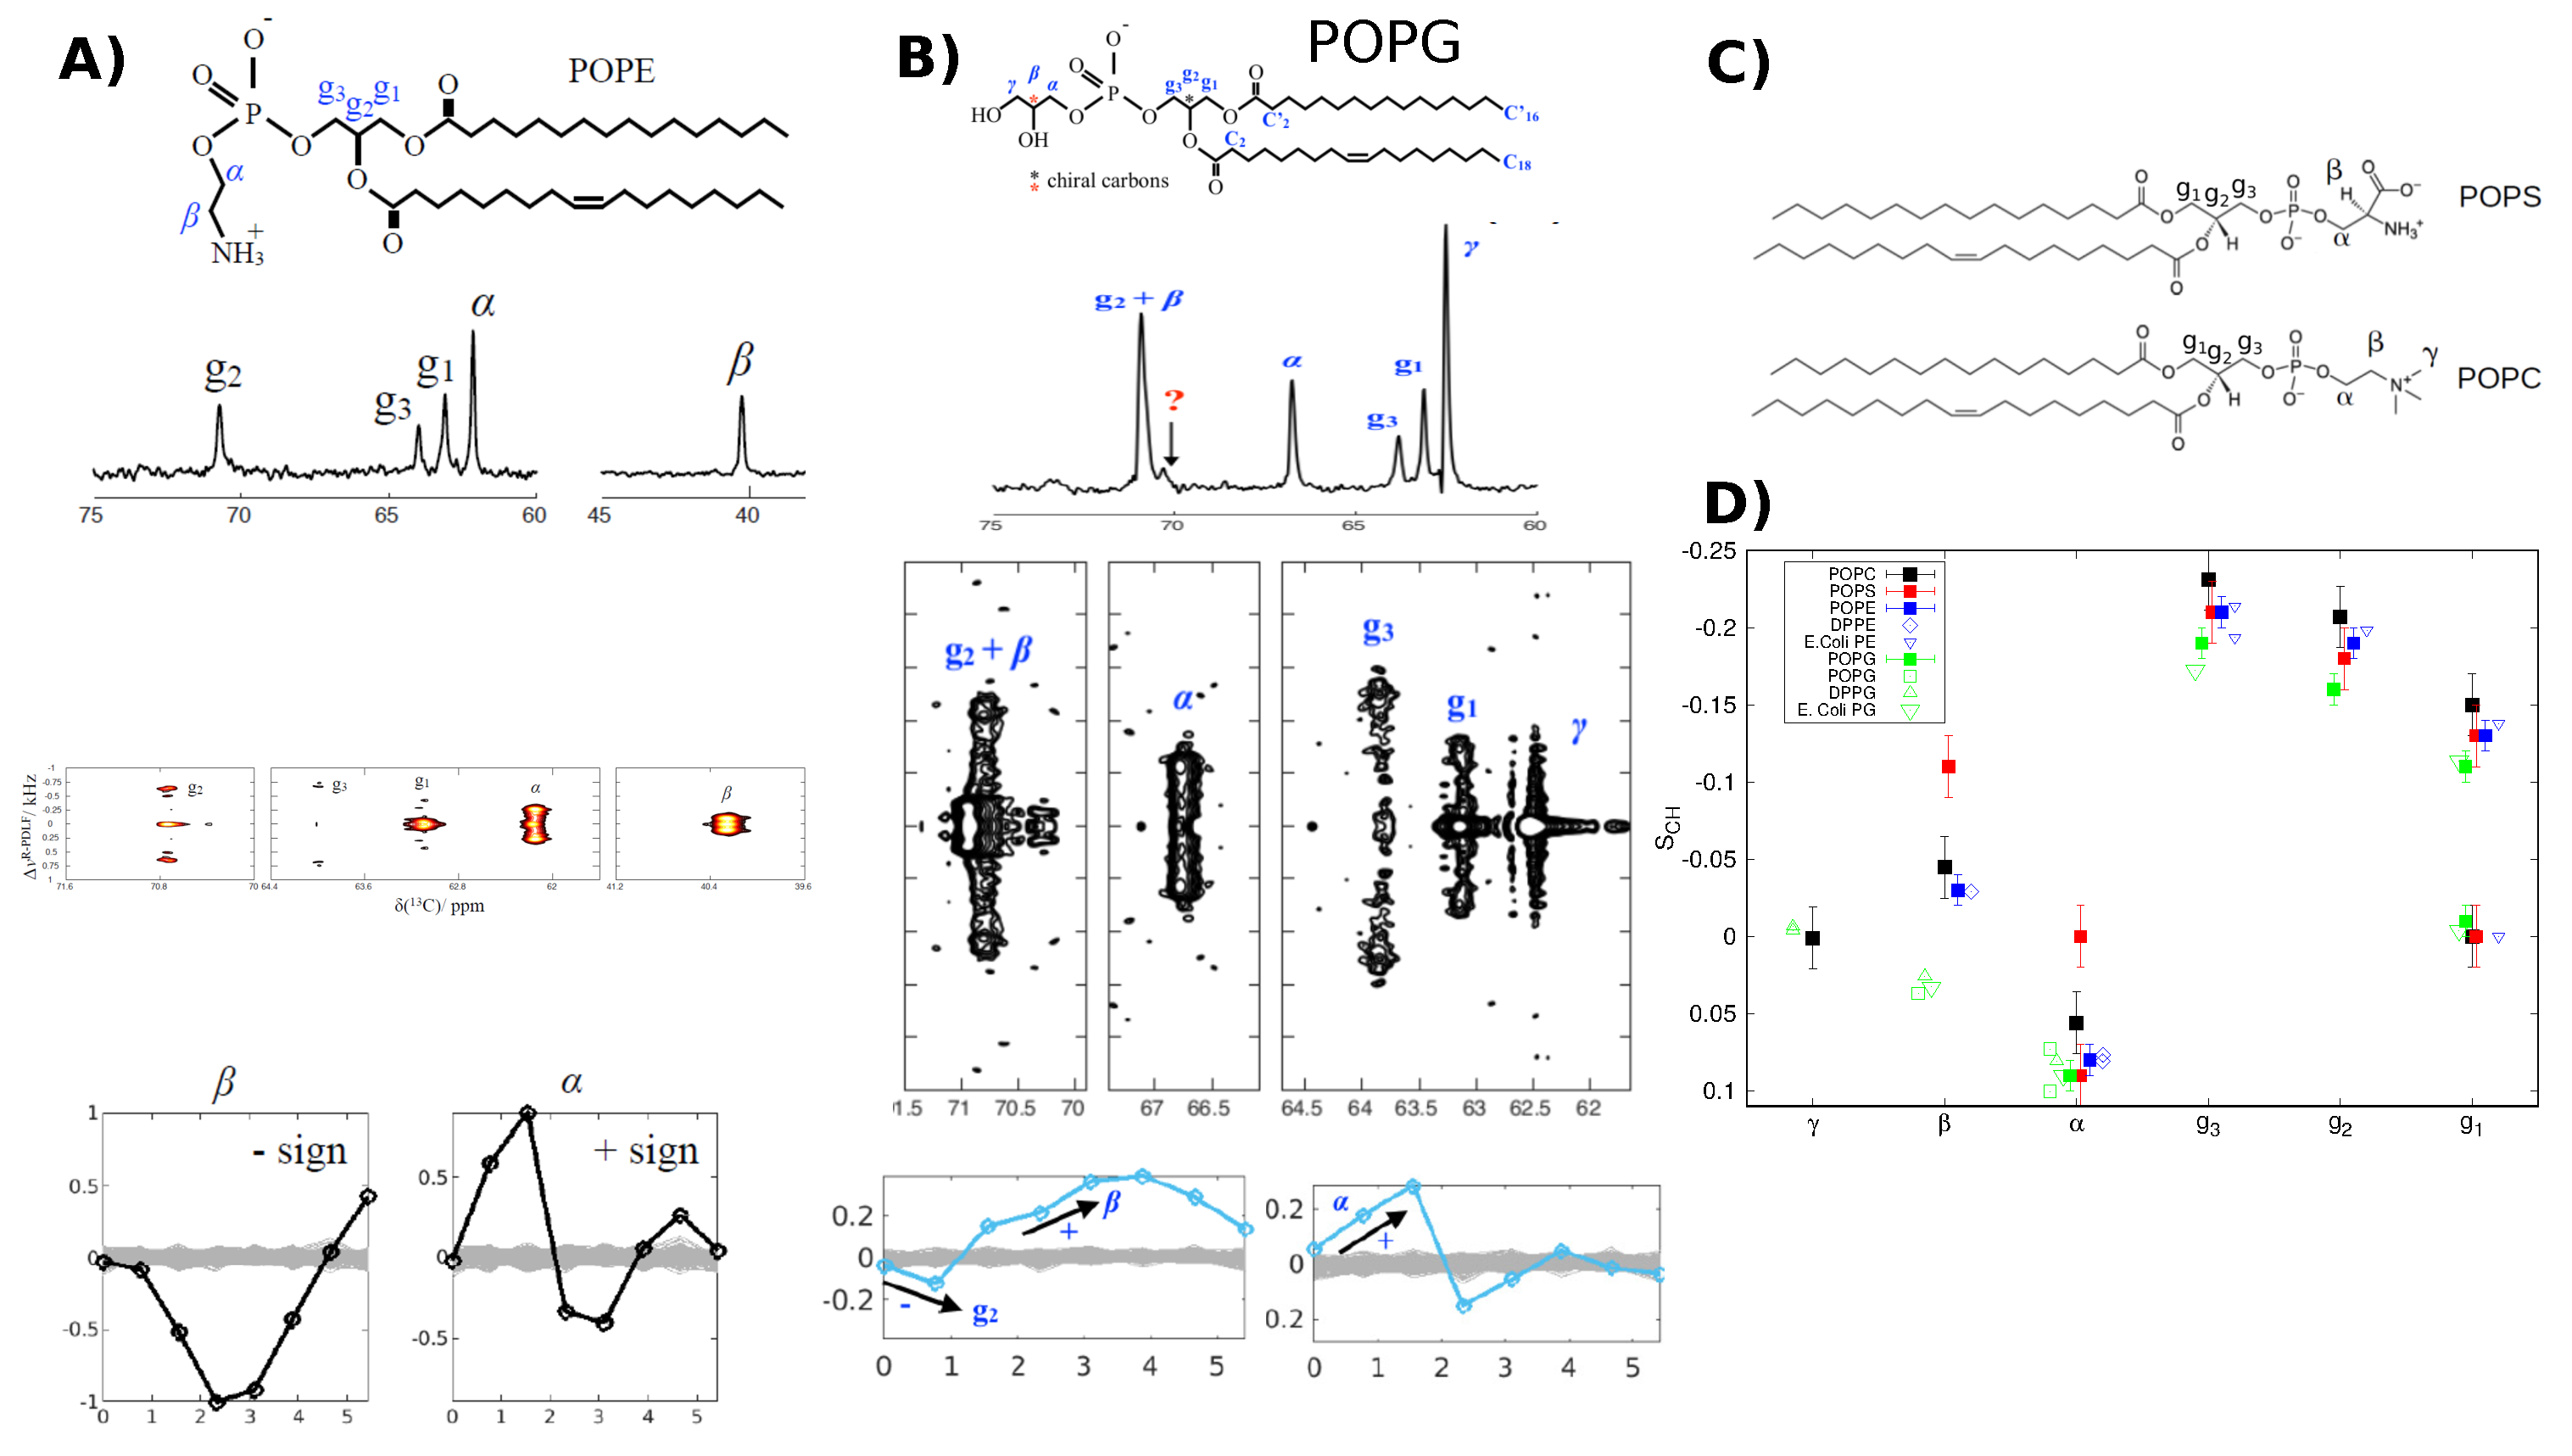
\includegraphics[width=18.0cm]{../Figs/figure1.eps}
   \caption{\label{HGorderParameters}
     Chemical structure, refocused-INEPT spectrum, 2D R-PDLF spectra, and S-DROSS data (from top to bottom) of {\bf A)} POPE  and {\bf B)} POPG.
    {\bf C)} Chemical structure of POPC and POPS.
    {\bf D)} Headgroup and glycerol backbone order parameters from different experiments in lamellar liquid disordered phase.
    The values and signs for POPE (310~K) and POPG (298~K)
    measured in this work, and for POPS (298~K) \cite{antila19} and POPC (300~K) \cite{ferreira13,ferreira16}
    previously using $^{13}$C NMR. The literature values for
    DOPS with 0.1M of NaCl (303~K) \cite{browning80},
    POPG with 10nM PIPES (298~K) \cite{borle85},
    DPPG with 10mM PIPES and 100mM NaCl (314~K) \cite{wohlgemuth80}, 
    DPPE (341~K) \cite{seelig76},
    E.coliPE and E.coliPG (310~K) \cite{gally81}
    are measured using $^2$H NMR. The signs from $^{13}$C NMR are used also for the literature values.
   }
   \todo{This is a sketch, needs a lot of polishing.} \\
  \todo{D) could be clarified as Fig. 2 in the NMRlipids IVps paper.}
\end{figure*}


\section{Results and Discussion}

%\subsection{Headgroup and glycerol backbone order parameters of POPE and POPG from $^{13}$C NMR}

\begin{figure*}[]
  \centering
   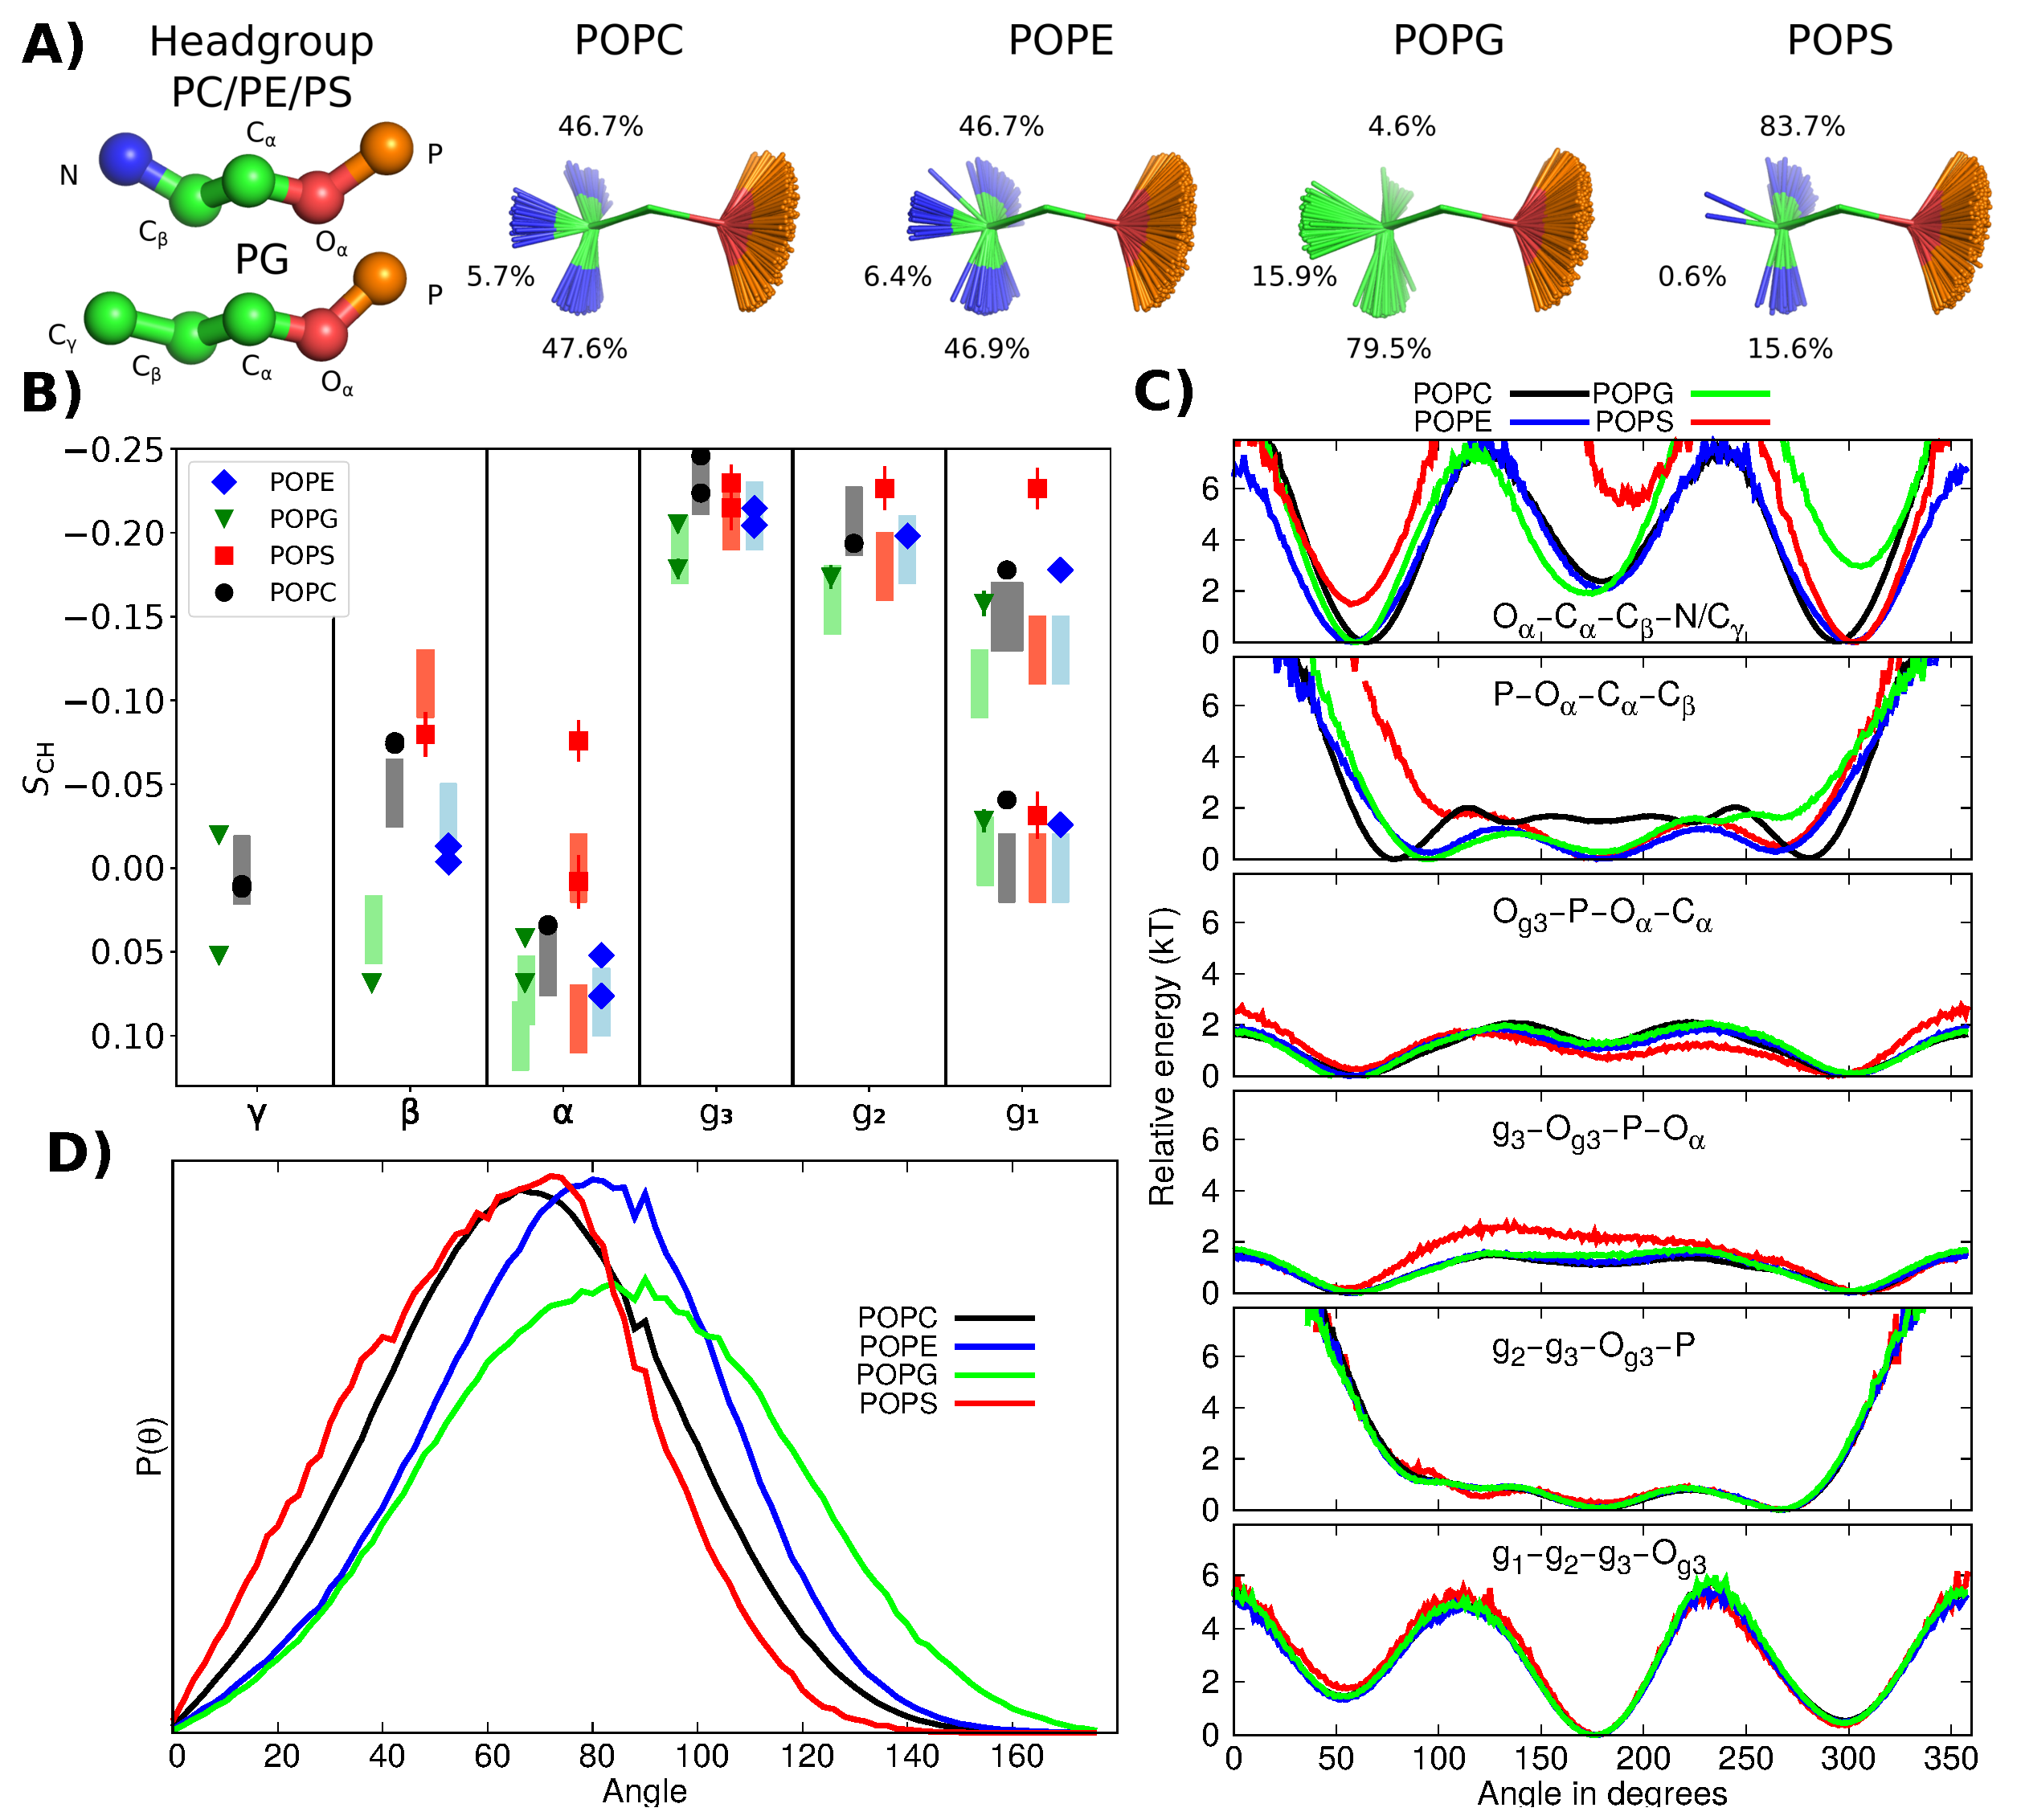
\includegraphics[width=18.0cm]{../Figs/figure2.eps}
%  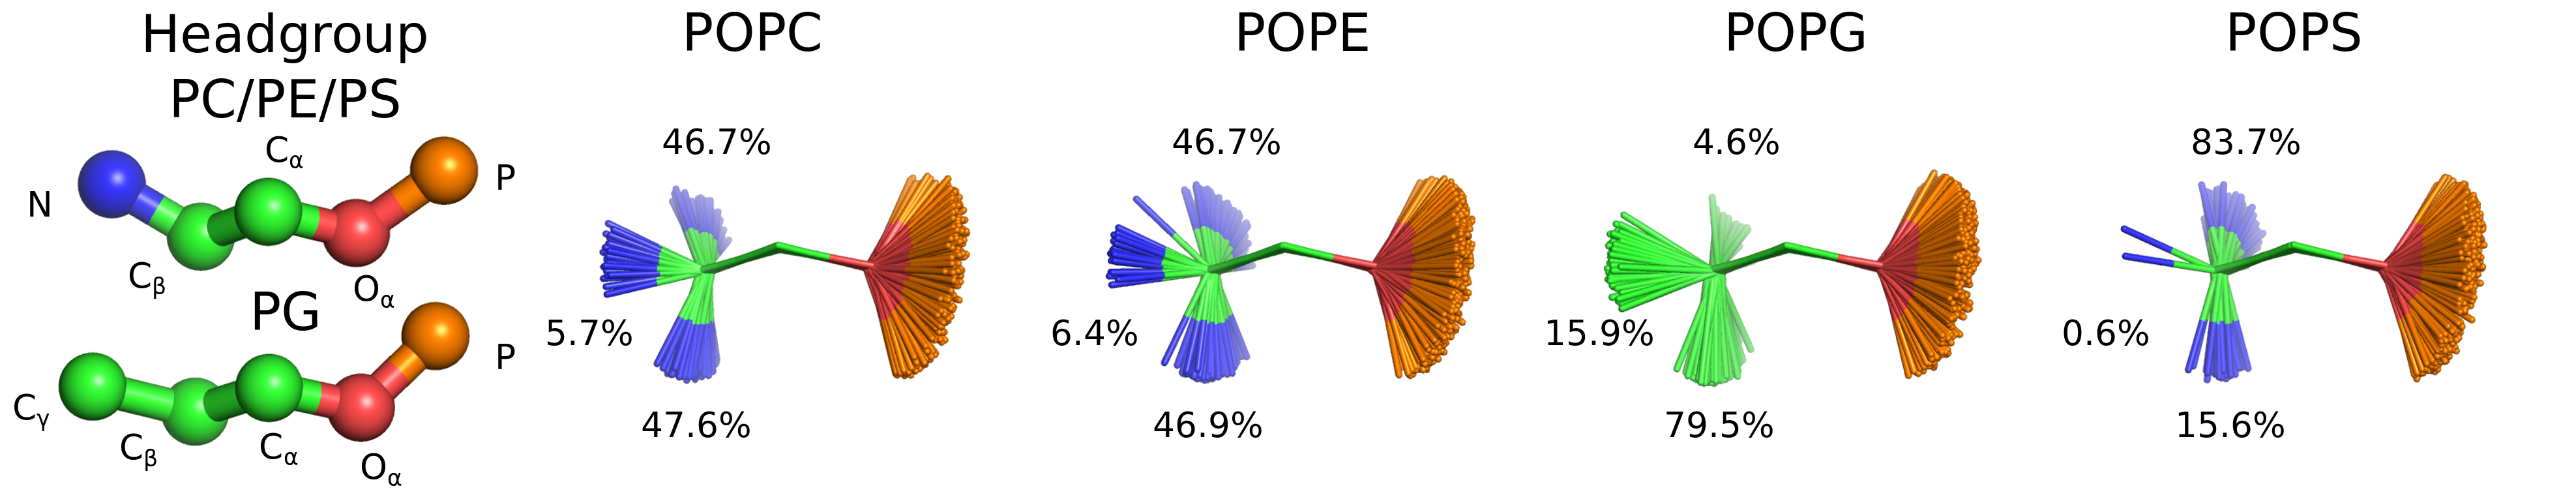
\includegraphics[width=18.0cm]{../Figs/PCPEPGPSstructures2.png}
%  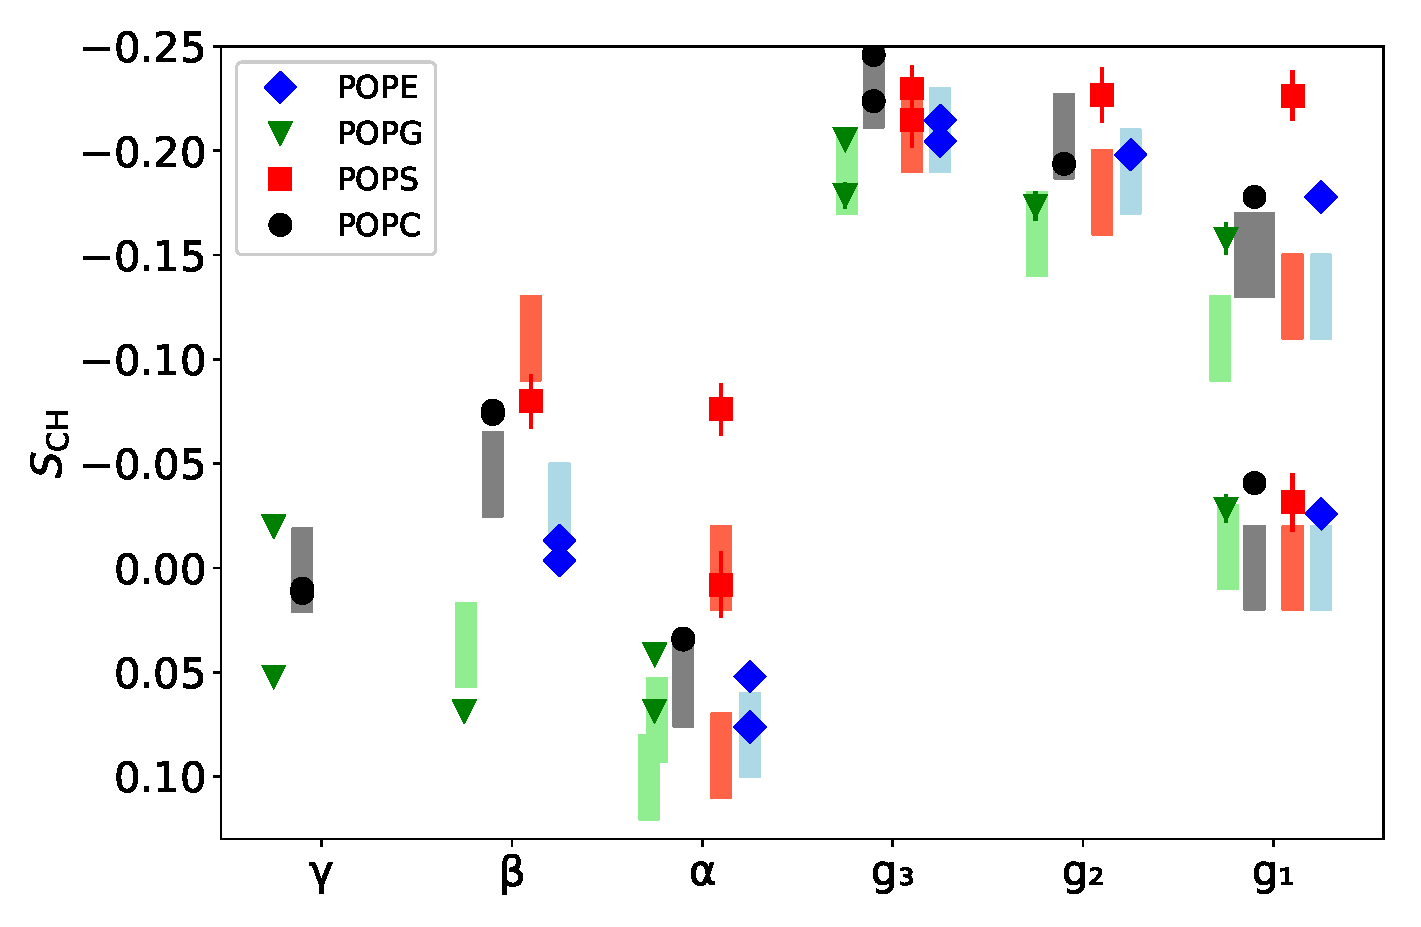
\includegraphics[width=8.0cm]{../Figs/CHARMMfromLIPIDS.eps}
%%  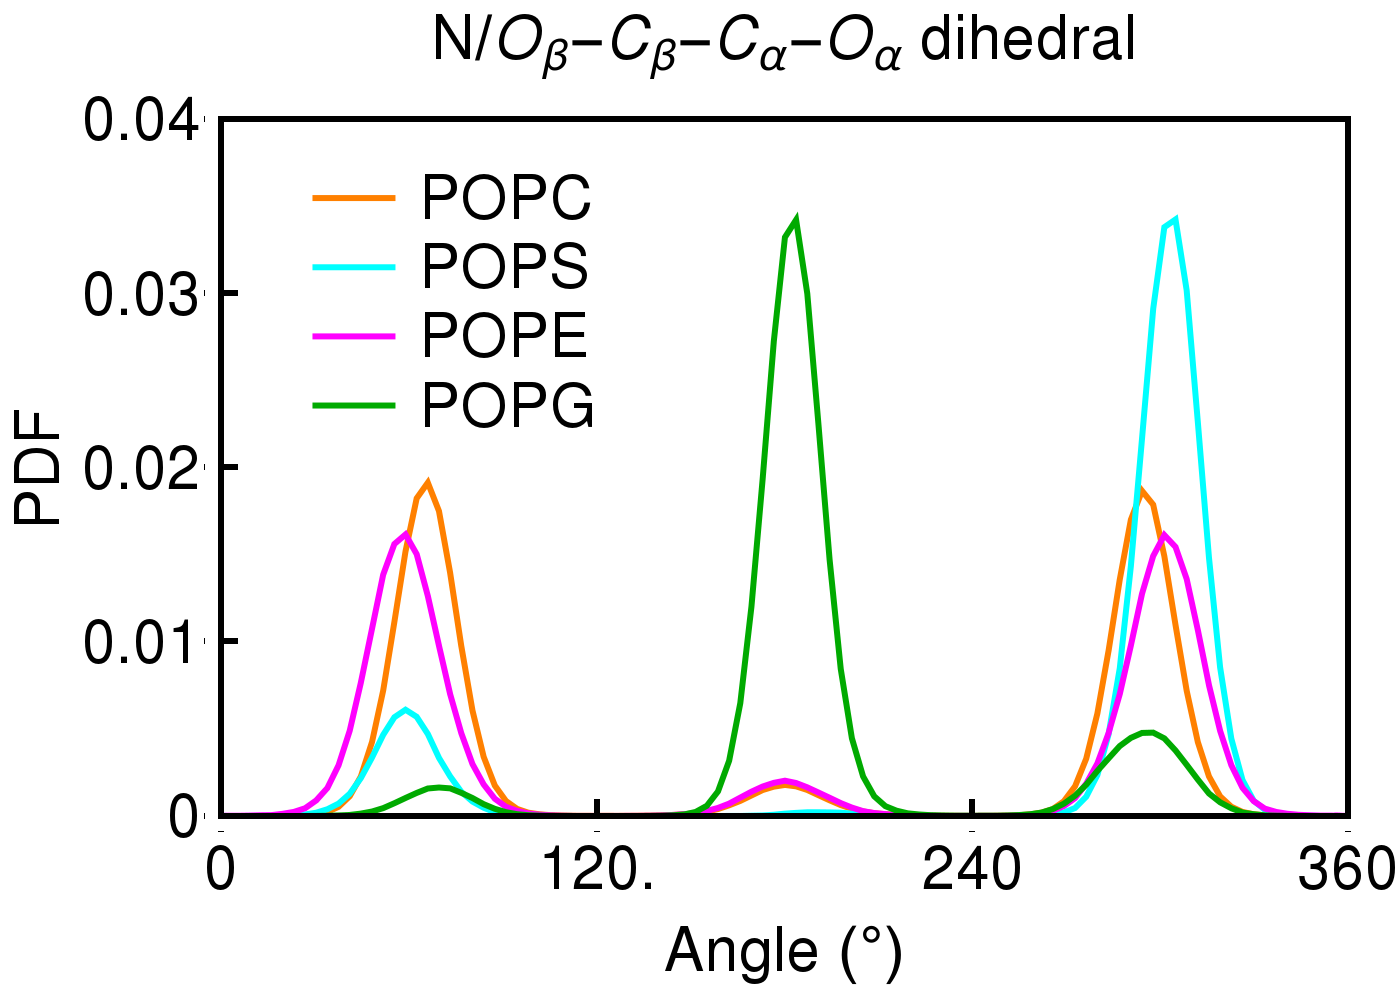
\includegraphics[width=8.0cm]{../Figs/PCPEPGPSdihedrals1.png}
%%  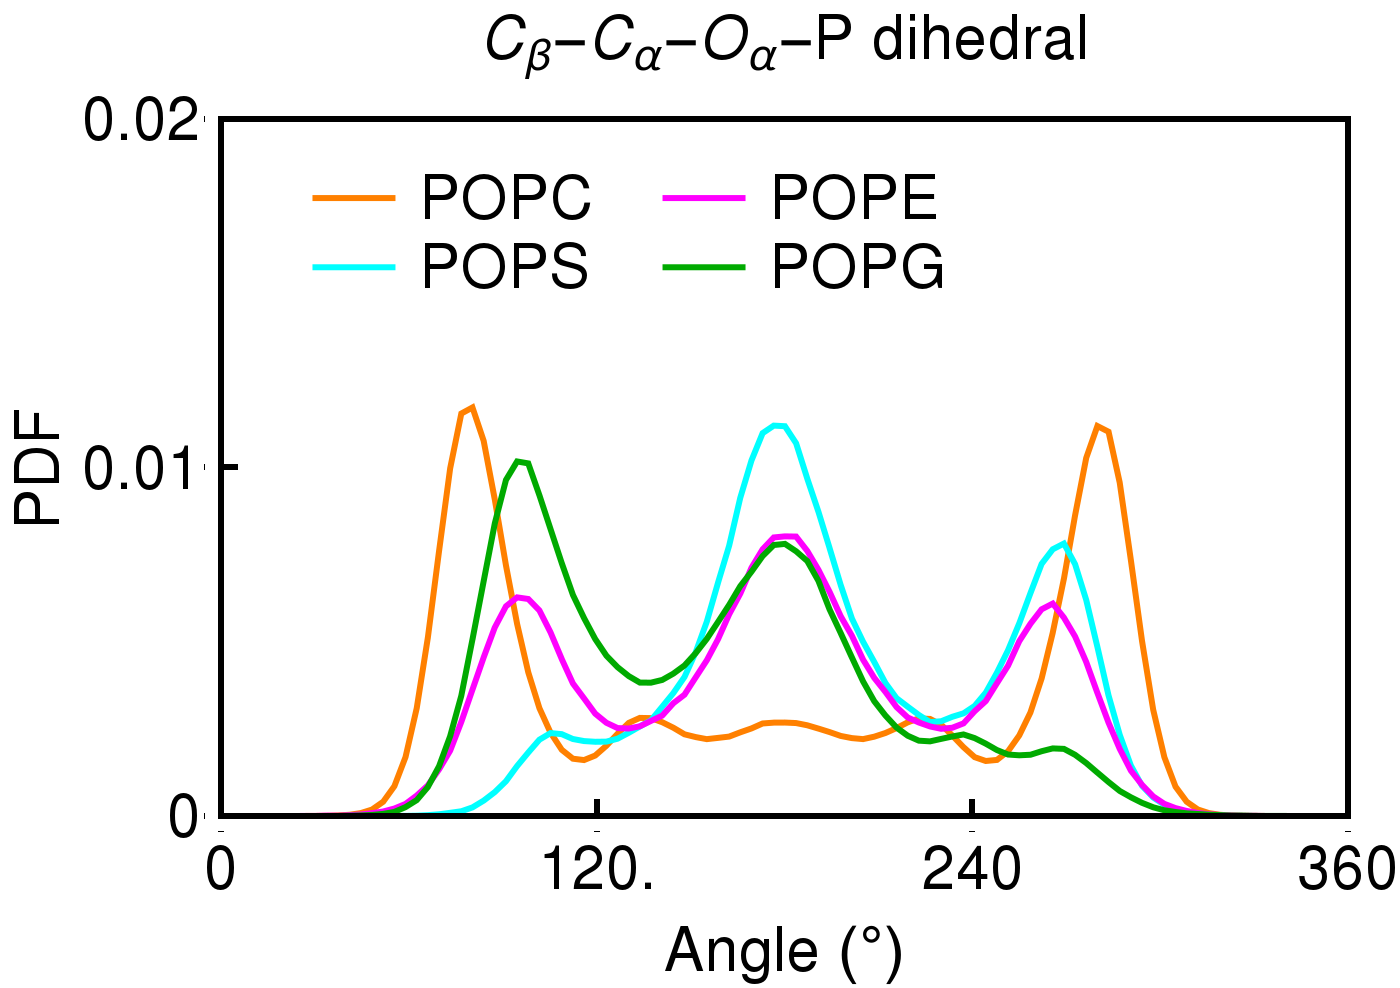
\includegraphics[width=8.0cm]{../Figs/PCPEPGPSdihedrals2.png}
%  \includegraphics[width=8.0cm]{../Figs/PNangleNORM.eps}
%  \includegraphics[width=8.0cm]{../Figs/DIHEDRALS.eps}
   \caption{\label{structures}
     Results from CHARMM36 simulations demonstrating the differences in conformational ensembles betwee different lipids. 
     {\bf A)} Snapshots with overlayed C$_\beta$, C$_\alpha$ and O$_\alpha$ atoms and occurence of different conformations.
     {\bf B)} Headgroup and glycerol backbone region order parameters of different different lipids.
     {\bf C)} Distributions of heavy atom dihedral angles of different lipids from CHARMM36 simulations.
     {\bf D)} Distributions of P-N vector angle with respect to membrane normal.
  }
  \todo{This is a draft and requires quite a bit of polishing.
    More detailed discussion of this figure is in https://github.com/NMRLipids/NMRlipidsIVPEandPG/issues/9} \\
\end{figure*}


\subsection{Conformational ensembles of different lipid headgroups in bulk bilayer}

To experimentally characterize the differences in lipid headgroup conformational ensembles
in liquid bilayer phase, we measured the C-H bond order parameters magnitudes and signs
from POPG and POPE bilayers.
Order parameters for POPE are in good agreement with previous $^2$H NMR experiments \cite{seelig76}
and similar to our previous results for POPC \cite{ferreira16}.
In POPG, the $\beta$ and g$_2$ carbons have similar chemical environment and their peaks
overlap in the NMR spectra (Fig. \ref{HGorderParameters} B).
The signs of these order parameters were solved using SIMPSON simulations to interpre the
S-DROSS experiments in similar fashion as we did previously for PS lipids \cite{antila19}.
The resulting order parameters are compared with our previously published results
for POPC \cite{ferreira13,ferreira16} and POPS \cite{antila19} in figure \ref{HGorderParameters} D.

%Our experimental order parameters, including the signs, from different lipid headgroups
%combined with the literature data are shown in Fig. \ref{HGorderParameters}.
%Also the headgroup order parameters of PC lipids are close PE, althought the latter gives systematically
%slightly more positive values (Fig. \ref{HGorderParameters}).
% These could be explained with slightly larger temperature in PE measurements, except for the $\alpha$-carbon with the positive sign, for which the
% more positive value is farther away from zero.
%While the headgroup order parameters are similar for PC and PE lipids,
%PG and PS lipids exhibit distinct values in comparison with other lipids.

The most distinct order parameters are observed for PS and PG headgroups.
In PS, the $\alpha$-carbon order parameter exhibits significant forking
and the $\beta$-carbon has more negative value than in other lipids.
In PG headgroup,
%the $\alpha$-carbon order parameter is similar to PE and PG, while
the $\beta$-carbon order parameter has positive sign in contrast to all the other lipids.
Notably, this has not been observed in traditional $^2$H NMR experiments,
%because absolute value of $\beta$-carbon order parameter is similar in PG, PE and PC lipids and
where only the absolute value of the order parameters are measured~\cite{wohlgemuth80,gally81,borle85}.
The glycerol backbone order parameters are similar for all the lipids, although they move slightly toward
positive values (closer to zero) in the order PC $<$ PE $<$ PS $<$ PG. 

%As discussed previously for PC and PS headgroups \cite{ollila16,antila19}, also 
%the headgroup and glycerol backbone order parameters of PE and PG are essentially independent of 
%acyl chain composition, and therefore manifest mainly headgroup chemistry (Fig. \ref{HGorderParameters}).

To characterize the differences in lipid headgroup conformational ensembles
leading to the distinct order parameters in PS and PG lipids, we calculate the
the distributions of heavy atom dihedral angles from CHARMM36 simulations.
Among available simulation models, this force field has least problems in
reproducing the experimental lipid headgroup and glycerol backbone order parameters in different
lipids \cite{botan15,antila19} (Figs. \ref{HGorderParametersPE} and \ref{HGorderParametersPOPG}).
Importantly, it captures the experimentally observed distinct order parameters for PS and PG headgroups (Fig. \ref{??}).
The dihedral distributions in figure \ref{structures} show significant similarity between different lipids for all the other
bonds, except for the last two bonds in the headgroup end, O$_\alpha$-C$_\alpha$ and  C$_\alpha$-C$_\beta$.
These differences explaing the disctinct order parameters of
PS and PG headgroups with respenct to the other lipids.
The difference between PC and PE lipids in the O$_\alpha$-C$_\alpha$ bond dihedral
may be an artefact because the $\beta$-carbon order parameter in PC is poorly reproduced by the CHARMM36 force field \cite{botan15}.
The differences between lipids are reflected also to the 
angle between headgroup dipole and membrane normal,
which decreases in the order of PG $>$ PE  $>$ PC  $>$ PS (Fig. \ref{structures}). 

%
%As in previous NMRlipids project results for PC and PS lipids \cite{botan15,antila19},
%none of the MD simulation force fields correctly captures all the
%headgroup and glycerol backbone order parameters of PE and PG lipids
%(Figs. \ref{HGorderParametersPE} and \ref{HGorderParametersPOPG})
%that would enable a straightforward interpretation of conformational ensembles.
%
%show wide variation between different force fields
%and none of the force fields reproduce all values within experimental error bars.
%(Figs. \ref{HGorderParametersPE} and \ref{HGorderParametersPOPG}),
%as observed previously also for PC and PS lipids \cite{botan15,antila19}.
%The Slipid simulations were able to capture the essential differences between PC and PS lipid
%headgroups \cite{antila19}, but this is not the case for PE and PG lipids.
%Without further discussion about poorly performing force fields, we focus on more detailed analysis
%of
%
%Nevertheless, CHARMM36 force field, which gives the results closest to the experiments for all lipids,
%captures the essential differences between
%PC, PS, PG and PE headroup order parameters  (Fig.~\ref{structures}) with the exception of $\beta$-carbon order parameter of PC
%
%give the best overall agreement with experiments for
%the headgroup and glycerol backbone order parameters of all PC, PS, PG and PE lipids in this and our previous
%studies \cite{botan15,antila19}. Even thought many order parameters in CHARMM36 simulations are
%not within the experimental error bars, it 
%
%which is too negative when compared with other lipids or experiments \cite{botan15}.
%
% As already pointed out in our previous study \cite{antila19},

The analysis of dihedral angle distributions reveal the free rotation of dihedral around
phosphorus-oxygen bonds in all lipids as all possible angles are observed in the distributions.
Results in figure \ref{structure} support the recently proposed models where this free rotation 
decouples the dynamics and conformational ensembles between acyl chains and headgroup in all lipids containing
the phosphorus group \cite{antila21}. 
However, some dihedral angles of phosphorus-oxygen bonds are less likely for PS, which
%suggests that the decoupling may be weaker for PS lipids
possibly explains the more rigid headgroup structures proposed for PS lipids~\cite{browning80,buldt81}.

%The eclipsed (0 or 360 degrees) are not present in any other dihedrals, and anti-eclipsed (120 or 240 degrees)
%are not present in C$_\alpha$-C$_\beta$ and g$_1$-g$_2$ bonds.


%Characteristic dihedral conformations in PS headgroup are asymmetric conformations
%preferring gauche 270$^\circ$ conformations in N-C$_\beta$-C$_\alpha$-O$_\alpha$ and
%%dihedral exhibits a more asymmetric angle distribution for PS, having largest probability being
%%in , than for the PC headgroup.
%C$_\beta$-C$_\alpha$-O$_\alpha$-P dihedrals. 
%In PG headgroup, the O$_\beta$-C$_\beta$-C$_\alpha$-O$_\alpha$ dihedral (corresponding N-C$_\beta$-C$_\alpha$-O$_\alpha$ dihedral in other% lipids)
%is mostly in trans conformation, and C$_\beta$-C$_\alpha$-O$_\alpha$-P  has asymmetric tendency to be in
%gauche 60$^\circ$ conformation. 
%Main difference between PC and PE is the lower probability of trans state in C$_\beta$-C$_\alpha$-O$_\alpha$-P PC dihedral,
%which could be a potential reason for the too negative $\beta$ headgroup order parameter in PC.%

\begin{figure*}[bt]
  \centering
  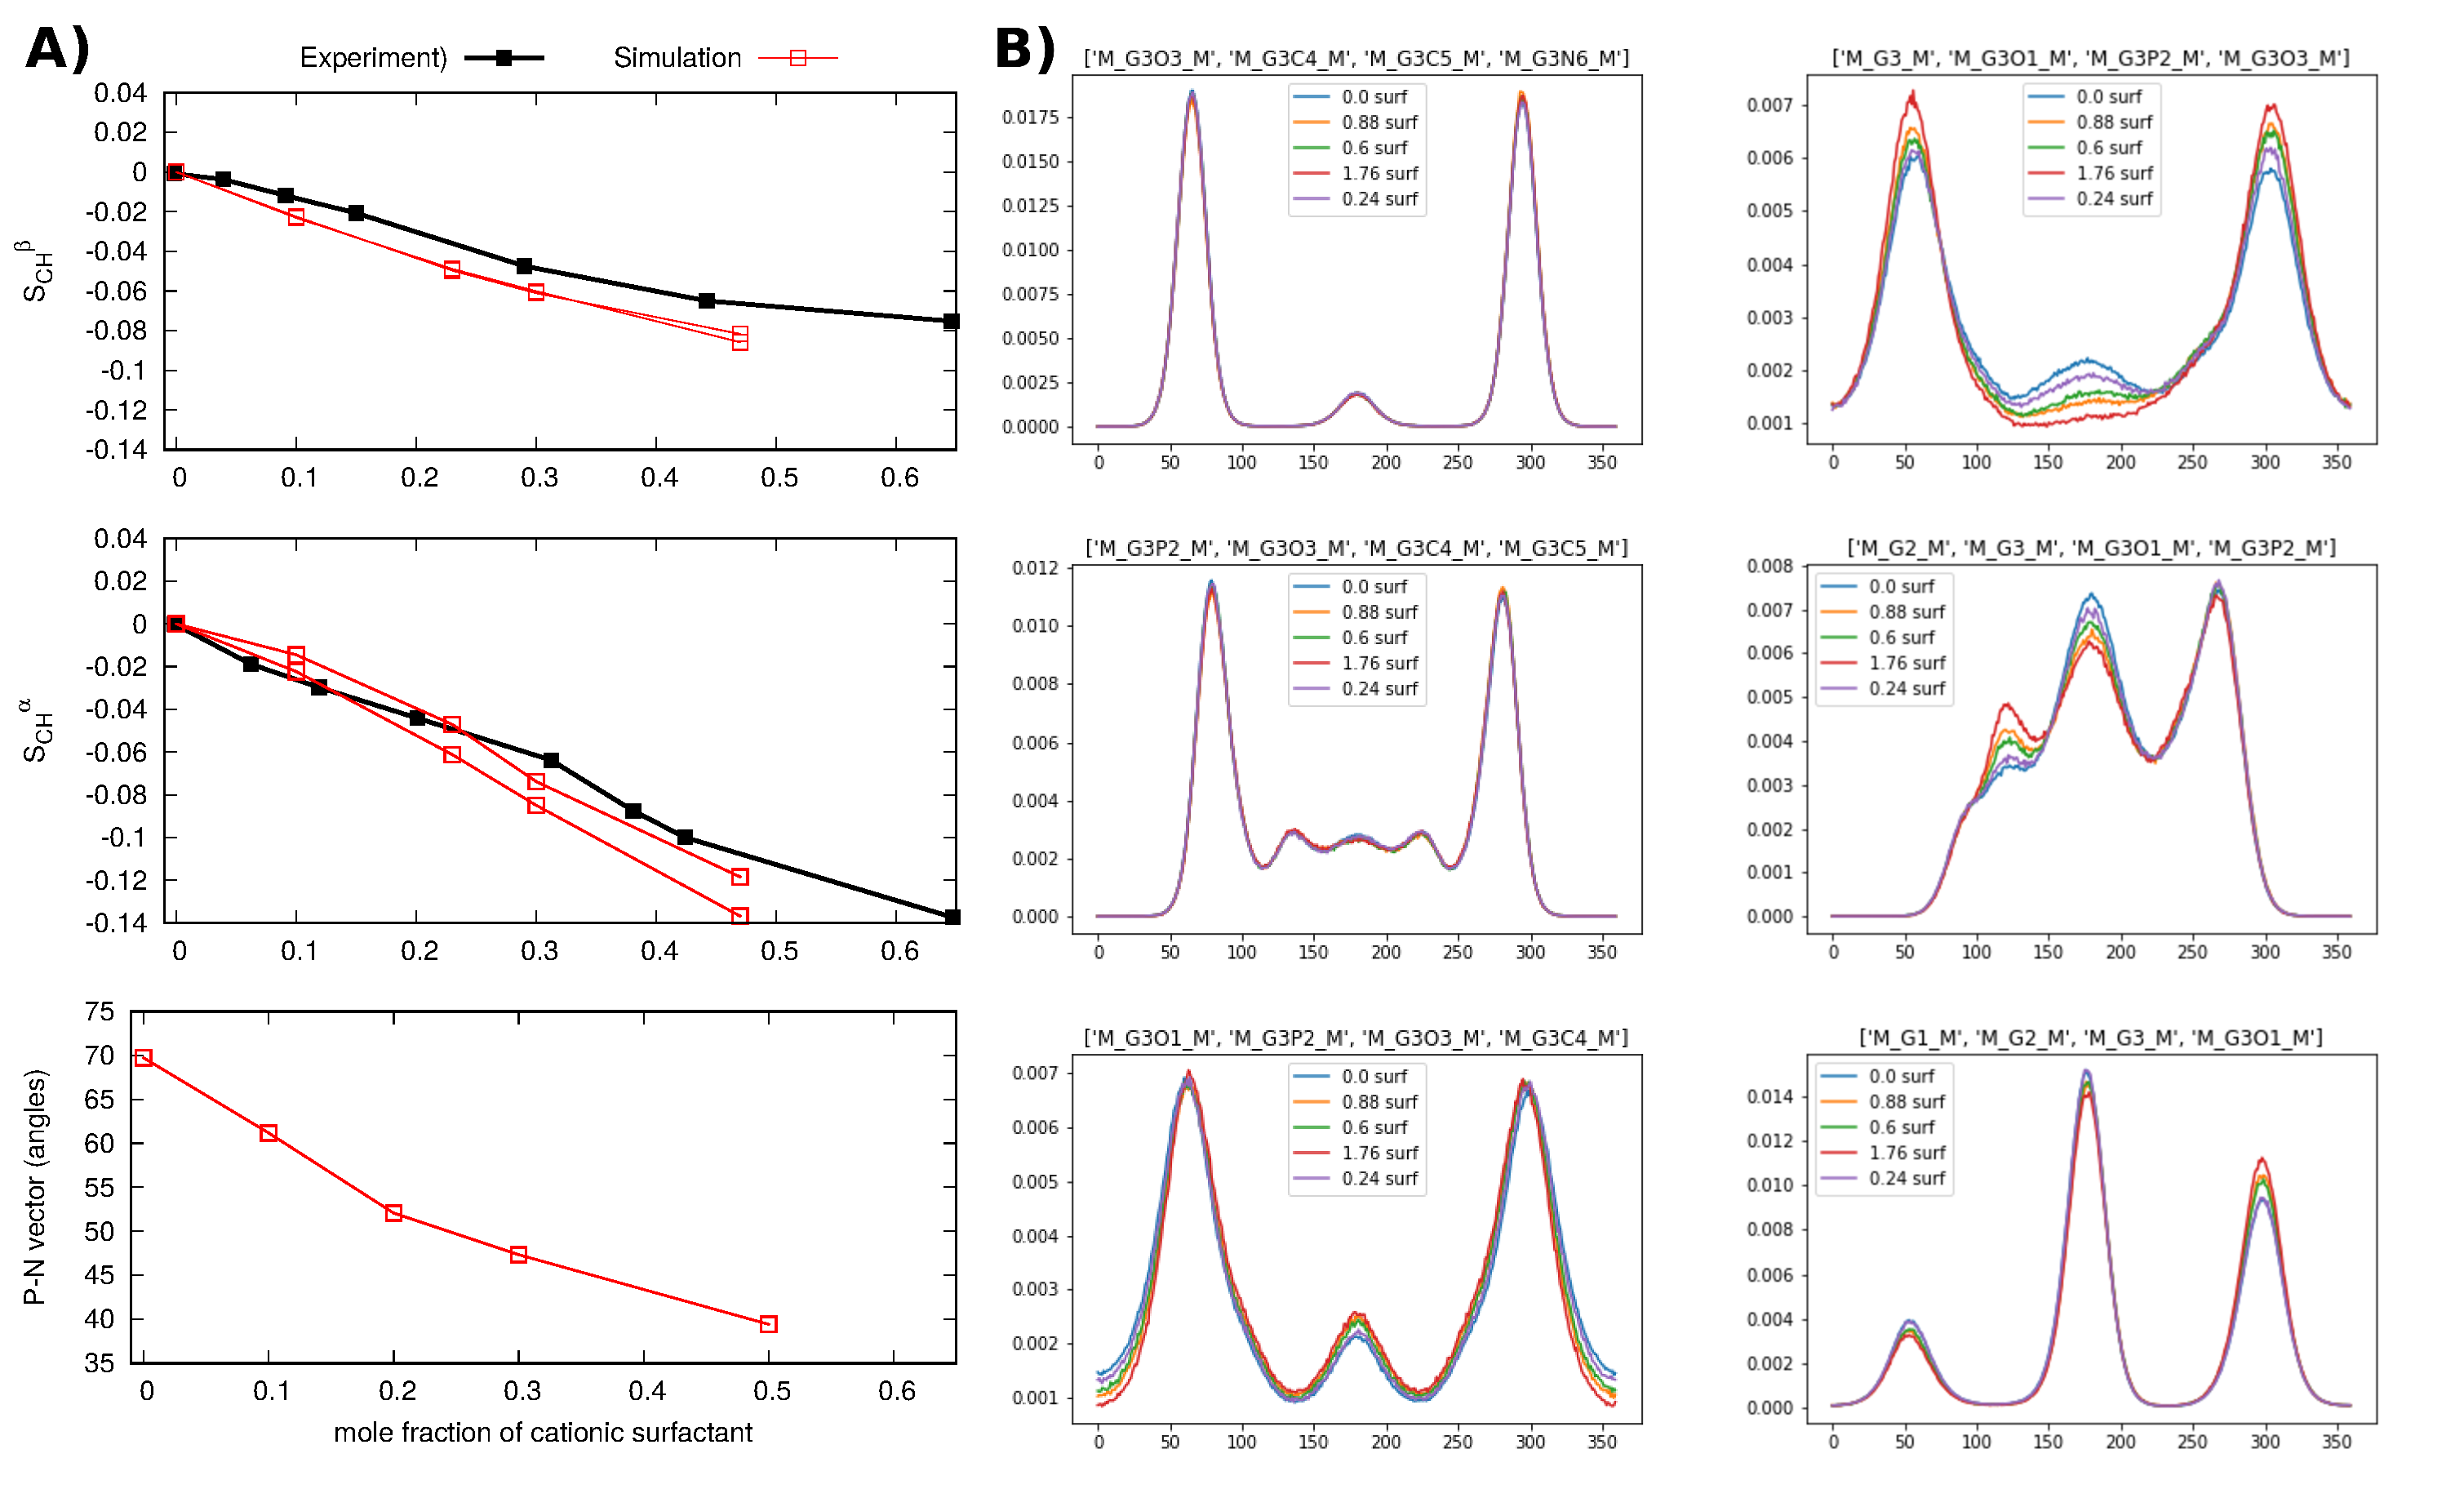
\includegraphics[width=18.0cm]{../Figs/figure3.eps}
  \caption{\label{changesWITHsurf}
    {\bf A)} Modulation of PC headgroup order parameters and P-N vector angle upon addition of cationic surfactant
    from CHARMM36 simulations compared with experimental data \cite{??}.
    {\bf B)} Changes in PC headgroup conformational ensembles upon increasing amount of positive charge in bilayer,
    characterized by the heavy atom dihedral distributions, from CHARMM36 simulations.
  }
\end{figure*}


In conclusion, all lipid headgroups sample very broad conformational ensembles in liquid lamellar phase.
%the results suggest that free rotations around O-P bonds decouple the
%headgroup and glycerol backbone structure and dynamics in similarly in all lipids,
%althought this rotation is slower in PS lipids where crossing certain barriers are slower.
Despite the differences in dihedral distributions of two the last bonds at the headgroup end,
leading to the distinct order parameters for PS and PG lipids,
lipids with different headgroup sample dihedral angles within approximately same ranges.
Altogether, our results suggest that lipid headgroups and very flexible thereby being
able to adopt multiple conformations when interacting with proteins, ions or other biomolecules.
Furthermore, approximately same conformations are present liquid lamellar phase for different
headgroups studied here, althought the probability weight for the conformations are slightly different.
%the order parameter experiments suggest that the glycerol backbone conformations in all lipids
%and the headgroup conformations in PC and PE lipids are relatively similar, while 
%PS and PG headgropus exhibit distinct conformational sampling.
%The details of sampled conformation are difficult to deduce from order parameters only,
%but the distinct headgroup order parameters
%of PS lipids are previously related to the more rigid structure of the headgroup~\cite{browning80,buldt81,antila19}.



\subsection{Lipid conformational ensembles in lipid bilayers with bound ions}
%Phosphatidylcholine headgroup conformational ensemble and orientation are unchanged
%upon addition of neutral molecules such as cholesterol or sphingomyelin into a bilayer,
%while
Order parameters of $\alpha$ and $\beta$ carbons in PC lipid headgroup are known to depend
linearly on the incorporation of charged molecules into a lipid bilayer,
which is explained by tilting of the headgroup dipole orientation \cite{??}.
%are kn affect the headgroup dipole vector tilt which can
%be detected by measuring C-H bond order parameters of $\alpha$ and $\beta$ carbons.
Such changes have been observed upon addition of charged lipids, proteins, surfactants,
drugs, or ions \cite{??}, but how charges affect the lipid conformational ensemble remains unknown.
%Headgroup order parameters of PC lipids decrease or increase upon addition of positive
%or negative charge into membrane, respectively, while they remain 
%\cite{??}.
%This has been explained by the tilting of the headgroup dipole due to electrostatic
%interactions with bound charges, and has been used to measure the binding affinity
%of ions to membranes \cite{??}.
%The headgroup order parameters of PC lipids can be used to measure the ion binding
%affinity to lipid bilayers because their magnitude is linearly proportional to the amount of bound charge in bilayer \cite{seelig87,catte16}.
%This molecular electrometer concept can be used also for bilayers containing PC lipids mixed with charged lipids \cite{borle85,macdonald87,roux90,antila19}.
%The headgroup order parameters can be used to evaluate MD simulations against experimental data,
%because they can be directly calculated from MD simulations \cite{catte16}.


%\begin{figure}[]
%  \centering
%  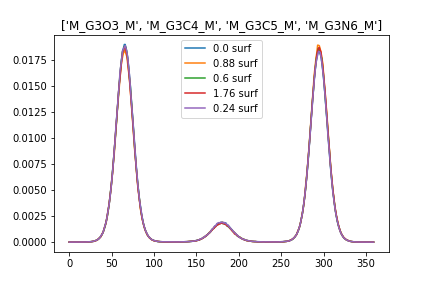
\includegraphics[width=6.0cm]{../Figs/dihedralFIGS/POPCsurf_M_G3O3_M_M_G3C4_M_M_G3C5_M_M_G3N6_MCHARMM36.png}
%  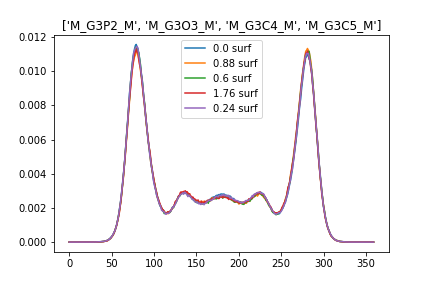
\includegraphics[width=6.0cm]{../Figs/dihedralFIGS/POPCsurf_M_G3P2_M_M_G3O3_M_M_G3C4_M_M_G3C5_MCHARMM36.png}
%  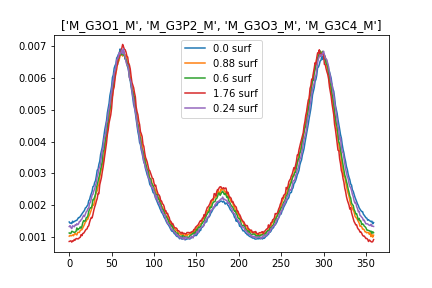
\includegraphics[width=6.0cm]{../Figs/dihedralFIGS/POPCsurf_M_G3O1_M_M_G3P2_M_M_G3O3_M_M_G3C4_MCHARMM36.png}
%  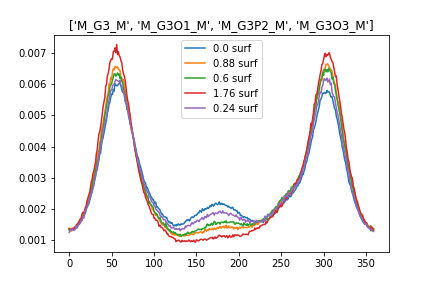
\includegraphics[width=6.0cm]{../Figs/dihedralFIGS/POPCsurf_M_G3_M_M_G3O1_M_M_G3P2_M_M_G3O3_MCHARMM36.png}
%  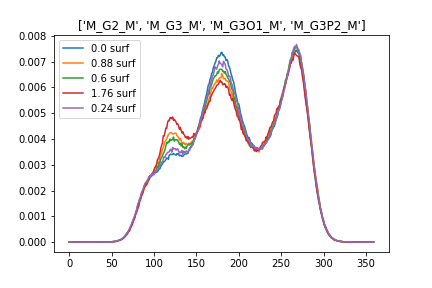
\includegraphics[width=6.0cm]{../Figs/dihedralFIGS/POPCsurf_M_G2_M_M_G3_M_M_G3O1_M_M_G3P2_MCHARMM36.png}
%  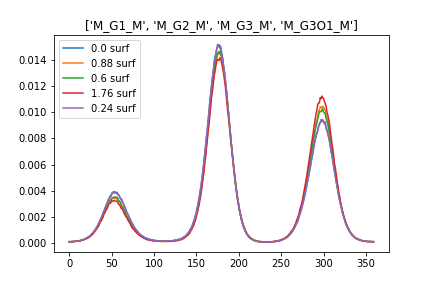
\includegraphics[width=6.0cm]{../Figs/dihedralFIGS/POPCsurf_M_G1_M_M_G2_M_M_G3_M_M_G3O1_MCHARMM36.png}  
%  \caption{\label{DIHSwithSURF}
%
%  }
%\end{figure}

The experimentally measured decrease of PC headgroup order parameters upon addition of cationic surfactants into a bilayer
are well captured by CHARMM36 simulations in figure \ref{changesWITHsurf} A,
suggesting that these simulations can be used to interpret how lipid headgroup conformational ensembles
respond to the binding of positively charged into a membrane.
Charactization of conformational ensembles using heavy atom dihedral angle distributions in figure \ref{changesWITHsurf} B
reveal that choline region is essentially unchanged upon addition of carge.
The major changes upon addition of charge are observed in dihedrals related to the phosphate oxygens,
while small change is observed also in the g$_2$-g$_3$ bond in the glycerol backbone.
This result is in line with the recently proposed model suggesting that the flexible phosphate enables the headgroup
orient according to the charge accumulated into a membrane \cite{antila21}.

\begin{figure*}[]
  \centering
  \includegraphics[width=18.0cm]{../Figs/CHANGESwithCaClPG1PC1.eps}
  \caption{\label{changesWITHCaClPG}
    Modulation of headgroup order parameters of POPC ({\it left}) and POPG ({\it right}) in POPC:POPG (1:1)
    mixture upon addition of CaCl$_2$ in 298 K temperature from experiments \cite{borle85,macdonald87} and simulations.
    The $\beta$-carbon order parameter of POPC (dashed line on top left) is not directly measured but
    calculated from empirical relation $\Delta S_{\beta}=0.43\Delta S_{\alpha}$ \cite{akutsu81}.
    The changes with respect to the systems without CaCl$_2$ are shown for other data than
    for the $\alpha$-carbon of POPG for which experimental order parameter is not available.
    Calsium density distributions are shown in figure \ref{CAdensPG}.
    %(right) The headgroup order parameters of PG from PC:PG mixtures as a function CaCl$_2$
    %concentration from experiments \cite{borle85} and CHARMM36 simulations.
  }
\end{figure*}


Headgroup order parameters of PC lipids respond similarly also to the addition of charged lipids in experiments \cite{??}.
To resolve the conformational ensembles of lipid headgroups also in biologically relevant
mixtures, % of zwitterionic and charged lipids,
we compared the response of headgroup order parameters in
PC lipids to the addition of PE or PG (Fig. \ref{??}),
as well as in PG lipids to the addition of PC (Fig. \ref{??}),
between simulations and experiments. However, the accuracy of currently available force fields
is not sufficient to capture the headgroup conformational ensembles
in mixed membranes: 
The best performing force field for single componen membranes, CHARMM36, overestimates
the effect of PE to PC conformations and underestimates the response PC to the addition
of anionic PG headgroup. Previously we explained similar result for PC/PS mixtures  
%as we previously observed also for mixtures with PS lipids \cite{antila19}.
%The latter may arise from
by overbinding of the sodium counterions \cite{antila19}.

In order to analyze how conformational ensemble of PC and PG lipids response to the
bound ions, we compared the changes of headgroup order parameters
in POPC:POPG (1:1) and (4:1) mixtures upon addition of CaCl$_2$ from different simulations
to the experimental data available in the literature \cite{borle85,macdonald87}
in figures \ref{changesWITHCaClPG} and \ref{changesWITHCaClPG1PC4}.
As in our previous studies \cite{catte16,melcr18,antila19,melcr20},  
%The decrease of POPC headgroup order parameters in mixtures with POPG lipids with
%increasing CaCl$_2$ concentration is overestimated in Slipids and Lipid17
%order parameters decrease in the response to bound cations in qualitative agreement with
%experiments, but
the calcium binding affinity to membranes is typically overestimated in simulations,
except by CHARMM36 with the NBfix correction which underestimates the binding affinity,
and the implicit inclusion of electronic polarizability improves the results.
Lipid17ecc model with the implicit inclusion of electronic polarizability gives
the most realistic response of PC lipid headgroup order parameters to the binding of calcium.
In this model, the main effect of calcium to the lipid conformational ensemble is
%the decrease is headgroup order parameters observed in this model is
the slight change of g$_3$-O$_{g3}$-P-O$_\alpha$ dihedral distribution from trans state
to eclipsed conformations (Fig. \ref{DIHSwithCAlipid17eccPOPC}).
This is in line with the changes observed in CHARMM36 simulations upon addition of charged surgactants (Fig. \ref{changesWITHsurf}),
despite the major differences in lipid headgroup conformational ensembles between
these models without ions (Fig. \ref{structures} vs. Fig. \ref{DIHSwithCAlipid17eccPOPC}).
%of lipid headgroup is not 
%Changes in lipid conformational ensembles characterized by distributions of heavy atom dihedral angles
%are very small upon binding of calcium or addition of cationic surfactants to membranes (Figs. \ref{??}).
%Yet, such changes are sufficient to tilt the headgroup dipole angle and reproduce the experimentally observed
%order parameter changes in $\alpha$ and $\beta$ carbons. 


%Among the available simulations, there are two models that correctly reproduce the
%PG headgroup order parameter changes upon addition of calcium, Lipid17 and Slipids,
%even though the binding affinity of calcium is overestimated in these simulations.
%The response of PC to calcium binding is correctly reproduced by Lipid17ecc model, as
%previously reported for other membranes \cite{melcr18,melcr19}.



%to Amber based lipid models
%improves the ion binding affinity leading to a good agreement with experiments.
%(Figs. \ref{changesWITHCaClPG} and \ref{changesWITHCaClPG1PC4})
%
%indicating too strong binding affinity of calcium into the bilayers as previously
%observed for pure PC lipid bilayers and mixtures with PS lipids \cite{catte16,antila19}.
%
%The decrease of $\alpha$-carbon order parameter of PC lipids in PC:PG mixtures as a function
%of calcium concentration is close to experiments CHARMM36 simulations (Fig. \ref{changesWITHCaClPG}),
%but the decrease of $\beta$-carbon order parameter seems to be overestimated.
%However, the $\beta$-carbon order parameter was not actually measured from these samples,
%but they are calculated from empirical relation $\Delta S_{\beta}=0.43\Delta S_{\alpha}$ \cite{akutsu81}.
%On the other hand, the simulations are not converged.
%
%The calcium binding affinity to lipid bilayers with PC and PS lipids
%was recently improved by applying the electronic continuum correction (ECC) to Amber Lipid14/17 force fields \cite{melcr18,melcr20}.
%In this approach, the electronic polarizability is implicitly included in the classical force fields
%by scaling the charges with constant factors \cite{leontyev11}. Here, we make a ECC-POPG force field
%by applying the scaling factors originally used for POPS also to POPG, i.e., we multiply
%charges and Lennard-Jones $\sigma$s of headgroup, glycerol backbone, and carbonyl regions with 
%$f_q$=0.75 and $f_\sigma$=0.89, respectively \cite{melcr20}.
%ECC-POPG model gives a weaker calcium binding affinity (Fig.\ref{CAdensPG}) and better agreement with the experimental
%PC headgroup order parameter changes (Fig. \ref{changesWITHCaClPG}) for POPC:POPG mixtures than the original Lipid17 model
%\todo{to be finished when we have all the data}, indicating that the ECC improves the simulation predictions of
%calcium binding affinity as previously observed for PC and PS lipids \cite{melcr18,melcr20}.



%\begin{figure}[]
%  \centering
%  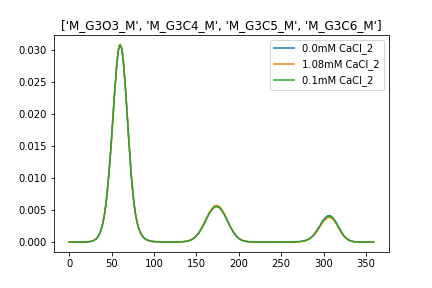
\includegraphics[width=6.0cm]{../Figs/dihedralFIGS/POPG_M_G3O3_M_M_G3C4_M_M_G3C5_M_M_G3C6_MCHARMM36.png}
%  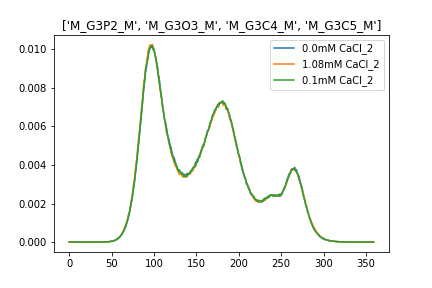
\includegraphics[width=6.0cm]{../Figs/dihedralFIGS/POPG_M_G3P2_M_M_G3O3_M_M_G3C4_M_M_G3C5_MCHARMM36.png}
%  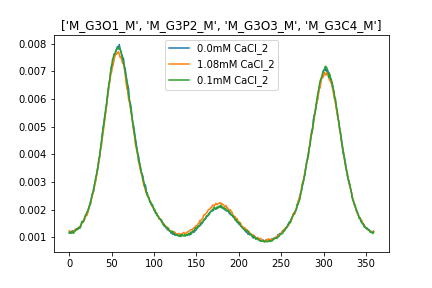
\includegraphics[width=6.0cm]{../Figs/dihedralFIGS/POPG_M_G3O1_M_M_G3P2_M_M_G3O3_M_M_G3C4_MCHARMM36.png}
%  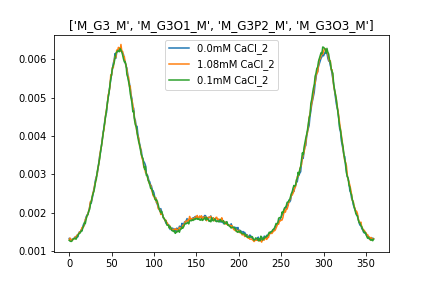
\includegraphics[width=6.0cm]{../Figs/dihedralFIGS/POPG_M_G3_M_M_G3O1_M_M_G3P2_M_M_G3O3_MCHARMM36.png}
%  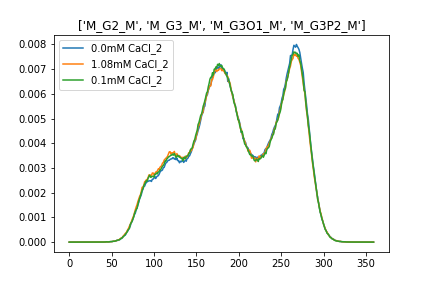
\includegraphics[width=6.0cm]{../Figs/dihedralFIGS/POPG_M_G2_M_M_G3_M_M_G3O1_M_M_G3P2_MCHARMM36.png}
%  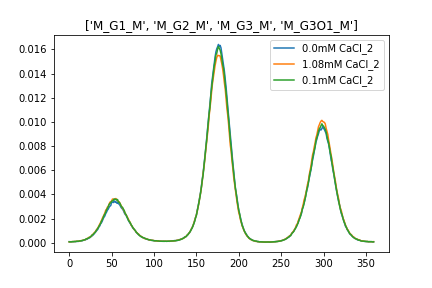
\includegraphics[width=6.0cm]{../Figs/dihedralFIGS/POPG_M_G1_M_M_G2_M_M_G3_M_M_G3O1_MCHARMM36.png}  
%  \caption{\label{DIHSwithCA}
%    Changes in POPG CHARMM36 dihedrals with increasing amount of CaCl$_2$.
%  }
%\end{figure}

%Simulations also qualitatively reproduce the experimentally observed decrease of POPG
%%Experimental data for the
%$\beta$-carbon order parameter
%%of POPG shows a rapid decrease with increasing
%upon addition of CaCl$_2$,
%%concentrations up to 10 mM
%suggesting that the PG headgroup response is qualitatively captured by simulations, in contrast
%to PS in our previous work \cite{antila19}.
%and more modest decrease with larger concentrations (Fig. \ref{changesWITHCaClPG}) \cite{borle85}.
%This behaviour is similar to that of $\beta$-carbon order parameters of POPC,
%but essentially different than observed for POPS, where $\beta$-carbon order parameters increases with
%addition of calcium \cite{antila19}. Experimentally measured changes of PG $\alpha$-carbon order parameters upon addition of
%calcium are not available.
%%upon addition of calcium in experiments,
%%exhibiting 
%%The behaviour is qualitatively different than in the $\beta$-carbon of PS lipids which increase upon addition of CaCl$_2$.

Decrease in headgroup order parameters of PC lipids upon addition of charges is
usually qualitatitely captured in simulations despite the inaccuries in lipid conformational ensembles \cite{catte16},
but situation with PS lipids is more complicated \cite{antila19,meclr20}.
Here, Lipid17 and Slipids force fields correctly capture the PG $\beta$-carbon order parameter response to CaCl$_2$
in figure \ref{changesWITHCaClPG} even thought the calcium binding affinity was overestimated.
%based on the comparison of PC headgroup order parameter changes with experiments.
%While applying ECC to Lipid17 improved the PC headgroup order parameter response and binding affinity,
%The response of PG $\beta$-carbon order parameter to calcium is too weak in CHARMM36 and ECC-lipid17 force fields,
%but decrease of the order parameter is associated with decreased P-N vector angle in all force fields.
Heavy atom dihedral angle distributions calculated from these simulations
%the changes in PG conformational ensemble from these models
suggest that also the headgroup glycerol conformations in PG are affected by calcium
(Figs \ref{DIHSwithCAslipidsPOPG} and \ref{DIHSwithCAlipid17POPG}),
in contrast to PC lipids where only conformations near phosphate were affected.
%dihedral angle distribution around O$_\alpha$-C$_\alpha$ bond is affected by calcium binding (Fig. ??).
On the other hand, the upward tilting of the headgroup dipole is weaker
%Even thought the change in headgroup orientation upon addition of calcium is smaller
in PG than in PC headgroup, possible due to the compensating effects from the changes in
phosphate and glycerol regions. 
However, none of the simulations captures and calcium binding affinity and conformational ensemble of PG lipids
simultaneously, and experimental data to evaluate 
%differences between force fields are observed for
the response of $\alpha$-carbon order parameters to
the added calcium in PG is not available.
Therefore, more accurate force fields are required for the solid analysis of PG conformations enembles in different ionic conditions.

%and PG
%The response of PG $\alpha$-carbon order parameters to CaCl$_2$ differs between force fields,
%but experimental data to evaluate these predictions is not available. 
%Simulations also qualitatively reproduce the experimentally observed decrease of POPG
%%Experimental data for the
%$\beta$-carbon order parameter
%%of POPG shows a rapid decrease with increasing
%upon addition of CaCl$_2$,
%%concentrations up to 10 mM
%suggesting that the PG headgroup response is qualitatively captured by simulations, in contrast
%to PS in our previous work \cite{antila19}.
%and more modest decrease with larger concentrations (Fig. \ref{changesWITHCaClPG}) \cite{borle85}.
%This behaviour is similar to that of $\beta$-carbon order parameters of POPC,
%but essentially different than observed for POPS, where $\beta$-carbon order parameters increases with
%addition of calcium \cite{antila19}. Experimentally measured changes of PG $\alpha$-carbon order parameters upon addition of
%calcium are not available.
%%upon addition of calcium in experiments,
%%exhibiting 
%%The behaviour is qualitatively different than in the $\beta$-carbon of PS lipids which increase upon addition of CaCl$_2$.


% The result is similar to the $\sim$200~ns simulations with PC lipids in previous work \cite{catte16}.
%However, when simulation was continued for $\mu$s, the binding affinity substantially increased
%and interpretation was that calcium overbinds to PC lipid in CHARMM36. Therefore, the
%conclusion seems to be similar here, although the new NBfix parameters may complicate
%the situation \todo{The status of NBfix parameters in these simulations should be checked.}.

%The $\beta$-carbon order parameter of PG exhibits a rapid decrease with small CaCl$_2$ concentrations
%and a more modest decrease with larger concentrations in experiments \cite{borle85} (Fig. \ref{PSPGchangesWITHCaCl}).
%The rapid decrease with CaCl$_2$ is observed but overestimated in CHARMM36 simulation
%with POPC:POPG 1:1 mixture, but not in 4:1 mixture \todo{This is little bit weird, should be checked.}.

%\todo{We still need more data to finish the discussion. More detailed discussion is in https://github.com/NMRLipids/NMRlipidsIVPEandPG/issues/12}

Despite the limited cabability of simulations to interpret some experimental data due to
the inaccuries in force fields, we can conclude that the experimentally observed changes
in headgroup order parameters upon addition of charges into bilayer arise from relatively
small changes in conformational ensembles. These changes can be characterised by
mild changes in dihedral angle distributions, rather than restriction of lipids into
fixed conformations. Therefore, lipid headgroups remain in disordered state sampling large
space of different conformations, thereby being able to interact with different molecules
in various ways, also when charged molecules are bound to membranes.



\subsection{Protein bound lipid conformations}

While our results in previous sections suggest that lipid headgroups
sample large conformational space in liquid lamellar phase, lipids
can bound to proteins in fixed conformations which can be then detected
using crystallography or cryo-EM. Such protein bound lipid conformations are
available within protein structures deposited in The Protein Data Bank (PDB)
available at \url{http://www.rcsb.org/} \cite{berman00}. With our criterias described
in the methods, we found
?? conformations of PC lipids,
?? conformations of PE lipids,
?? conformations of PG lipids, and
?? conformations of PS lipids from PDB.

\begin{figure}[]
  \centering
  \includegraphics[width=8.0cm]{../Figs/DIHEDRALSALLfromPDB.eps}
%  \includegraphics[width=8.0cm]{../Figs/DIHEDRALSPEfromPDB.eps}
%  \includegraphics[width=8.0cm]{../Figs/DIHEDRALSPGfromPDB.eps}
%  \includegraphics[width=8.0cm]{../Figs/DIHEDRALSPSfromPDB.eps}
  \caption{\label{dihedralsFROMpdb}
    Dihedral distributions from simulations and lipid structures in PDB.
  }
\end{figure}

To analyze the relation of lipid headgroup conformational ensembles between
liquid lamellar and protein bound states, we calculated the heavy atom dihedral angle
distributions also from the protein conformations found from the PDB.
The results in figure \ref{dihedralsFROMpdb} do not reveal major differences
between different lipid headgroups when bound to proteins.
Some preference for trans state in C$_\alpha$-C$_\beta$ bond of PC lipids, and
for positive angles in O$_\alpha$-C$_\alpha$ and P-O$_\alpha$ of PS lipids with respect
to other lipids may be present in the data, but more statistics is required for solid
conclusions. Therefore, the differences in conformational ensembles between different
lipids observed in liquid lamellar state are not clearly visible in the protein bound states.

Almost all dihedral angles are found from the protein bounds states for all dihedrals
except for P-O$_\alpha$-C$_\alpha$-C$_\beta$ and g$_2$-g$_3$-O$_{g_3}$-P, which seem to avoid
the cis conformations. The wide range of available dihedrals is similar to our results
in liquid lamellar state, except for O$_\alpha$-C$_\alpha$-C$_\beta$-/C$_\gamma$ and
g$_1$-g$_2$-g$_3$-O$_{g_3}$ dihedrals which seem to be more restricted in the liquid
lamellar phase (Fig. \ref{structures}). This suggests that lipids compromize their
preferred conformations when bound to proteins to minimize the intermolecular interactions
with proteins.

\section{Conclusions}

We have measured the C-H bond order parameters with the signs for headgroup and glycerol
backbone regions of the most most abundant biological phopholipids, PC, PE, PG and PS.
Combining this experimental data with the large amount of simulation data collected 
using the NMRlipids open collaboration, we were able to resolve the differences between
conformational ensembles of lipid headgroup leading to the differences observed in NMR experiments.

Our results indicate that lipid headgroups are flexible and sample large conformational space
in biologically relevant liquid lamellar state, also in membranes containing charged molecules,
which have the largest affect on lipid headgroups in NMR experiments.
Therefore, lipids can bind to proteins and other biomolecules in multiple different conformations,
as indeed observed in the analysis of protein bound lipid conformations available from PDB.
The weak correlation between lipid structures in liquid lamellar phase and protein bound state
suggestst that the selective lipid binding to proteins is dominated by the intermolecular lipid-protein
interactions, and the differences in conformational ensembles between different lipid types
play only a minor role.

Our results pave the way to understand how lipids regulate membrane protein function.
For example, the resolved lipid conformational ensembles in liquid lamellar phase and
realistic MD simulations enables accurate analysis of lipid-protein interactions energetics.
Furthermore, our results demonstrate how NMR data can be combined with the large amount of
indexed MD simulation data to find the most realistic conformational ensembles of biomolecules
in membrane environment. This paves the way toward standardized methods to resolve the quality
evaluated conformational ensembles of disordered biomolecules in membrane environment.
In the NMRlipids project we aim to build a general databank of quality evaluated
conformational ensembles of lipids and other disordered biomolecules based primarily on
MD simulations and NMR data.



% Tables may be be put in the text as floats.
% Here is an example of the general form of a table:
% Fill in the caption in the braces of the \caption{} command. Put the label
% that you will use with \ref{} command in the braces of the \label{} command.
% Insert the column specifiers (l, r, c, d, etc.) in the empty braces of the
% \begin{tabular}{} command.
%
% \begin{table}
% \caption{\label{} }
% \begin{tabular}{}
% \end{tabular}
% \end{table}

% If you have acknowledgments, this puts in the proper section head.
\begin{acknowledgments}
AP is grateful to the Centro de
Supercomputación de Galicia (CESGA) for use of the Finis
Terrae computer
    %     Put your acknowledgments here.
\end{acknowledgments}
%\newpage
%\appendix
%\begin{center}
%{\bf SUPPLEMENTARY INFORMATION}
%\end{center}



%\section{Measurements of order parameter sign}

%Fig. \ref{PShgSIGNS} summarizes the experimental results on the order parameter sign
%measurement for POPS sample. The experimental protocol is the same used in Ref. \citenum{ferreira16}.
%In (a) you see the headgroup region of the INEPT spectrum where alpha and beta are
%identified. In (b) you have the R-PDLF slices for alpha and beta where you see one single
%splitting for beta (which gives an order parameter equal to 0.12), and for alpha a superposition
%of a large splitting (order parameter equal to 0.09) and a very small splitting which cannot be
%calculated. On the bottom you have the S-DROSS slices of these two carbons. The grey lines show a
%random collection of slices from noise such that it gets clear what is significant. The S-DROSS
%slice for beta clearly shows that the order parameter is negative. The slice for alpha shows that
%the higher order parameter is positive and suggests that the smaller order parameter is negative
%(from the deviation towards negative values in the longer t1 times).
%\begin{figure}[]
%  \centering
%  \includegraphics[width=9.0cm]{../Figs/PShgSIGNS.pdf}
%  \caption{\label{PShgSIGNS}
%    Experimental results for sign measurement for POPS sample
%  }
%\end{figure}

%The results updated with SIMPSON simulations for the SDROSS profiles
%are shown in Fig. \ref{PShgSIGNSsimpson}. The value for the smaller
%alpha order parameter is taken from Fig 3 in Ref. \citenum{roux91},
%because resolution in 13C NMR experiments was nor high enough to determine
%numerical value for this. The plots in Fig. \ref{PShgSIGNSsimpson} (c) show
%the following. The error bars and points are the experimental SDROSS data.
%The thick lines are SIMPSON simulations. The simulations were done by using
%the order parameter for beta equal to -0.12 and for alpha one order parameter
%equal to 0.09 and the other equal to -0.02 (black) or 0.02 (grey).
%Since the black lines agree with experimental data, we conlude that
%the order parameters for $\beta$ carbon are -0.12 and for $\alpha$
%order parameters are 0.09 and -0.02.
%\begin{figure}[]
%  \centering
%  \includegraphics[width=9.0cm]{../Figs/PShgSIGNSsimpson.pdf}
%  \caption{\label{PShgSIGNSsimpson}
%    Experimental results for sign measurement for POPS sample
%  }
%\end{figure}

%\section{Dihedrals}
%\begin{figure*}[]
%  \centering
%  \includegraphics[width=8.0cm]{../Figs/dihed1.png}
%  \includegraphics[width=8.0cm]{../Figs/dihed2.png}
%  \includegraphics[width=8.0cm]{../Figs/dihed3.png}
%  \includegraphics[width=8.0cm]{../Figs/dihed4.png}
%  \includegraphics[width=8.0cm]{../Figs/dihed5.png}
%  \includegraphics[width=8.0cm]{../Figs/dihed6.png}
%  \includegraphics[width=8.0cm]{../Figs/dihed7.png}
%  \includegraphics[width=8.0cm]{../Figs/dihed8.png}
%  \includegraphics[width=8.0cm]{../Figs/dihed9.png}
%  \includegraphics[width=8.0cm]{../Figs/dihed10.png}
%  \caption{\label{dihedrals}
%    Experimental results for sign measurement for POPS sample
%  }
%\end{figure*}

% Create the reference section using BibTe
\bibliography{refs.bib}

%\newpage
%\section{APPENDIX: The NMR results reported by Tiago Ferreira}

\listoftodos

\end{document}
%
% ****** End of file aiptemplate.tex ******
